
\chapter{Man in the middle Attacks}
\newpage

\section{lecture}
Let me explain both attack types:

A Man-in-the-Middle (MITM) attack is where an attacker secretly intercepts and potentially alters communications between two parties who believe they're directly communicating with each other. Here's how it typically works:

\begin{enumerate}
	\item Alice wants to communicate with Bob
	\item Mallory (the attacker) intercepts the connection
	\item Mallory creates two separate connections - one with Alice and one with Bob
	\item Alice thinks she's talking directly to Bob, and Bob thinks he's talking directly to Alice
	\item Mallory can read and modify all messages passing between them
\end{enumerate}

Common MITM scenarios include:
\begin{enumerate}
	\item Intercepting traffic on unsecured public WiFi
	\item DNS spoofing to redirect users to malicious servers
	\item SSL stripping to downgrade HTTPS to HTTP
	\item ARP spoofing on local networks
\end{enumerate}

Man-in-the-Browser (MitB) is a more sophisticated variant that operates at the browser level rather than the network level. It typically works by:

\begin{enumerate}
	\item Installing malware that hooks into the web browser (often via browser extensions or trojans)
	\item Monitoring and modifying web pages in real-time before they're displayed to the user
	\item Intercepting data before it's encrypted and sent to legitimate websites
	\item Modifying transaction details while maintaining a legitimate-looking display to the user
\end{enumerate}

MitB attacks are particularly dangerous because they can:
\begin{itemize}
  \item Bypass HTTPS encryption since they operate after decryption
  \item Modify both what the user sees and what they send to websites
  \item Be very difficult to detect since they show legitimate SSL certificates
  \item Override security mechanisms like two-factor authentication
\end{itemize}

The key difference is that MITM operates at the network level by intercepting traffic between points, while MitB operates inside the browser itself, manipulating data before encryption or after decryption.

Would you like me to elaborate on any particular aspect of these attack types?

\textbf{Attacks discussed in lecture:}
\begin{itemize}
  \item MITM
  \item MitB
  \item via forged BGP
  \item at border control with IMSI Catcher
  \item 2g/3g/4g Rouge antenna - IMSI Catcher
  \item @Home of Suspect 
  \begin{itemize}
    \item Mobile Network
    \item ISP
  \end{itemize}
  \item WIFI network, Rouge Access Point - WiFi Pineapple
  \item NFC - used for payments
  \item WIFI Bluetooth
  \item arp spoofing
  \item DHCP poisoning
  \item With Malware/GovWare
  \item DNS poisoning
  \begin{itemize}
    \item hosts file
    \item with proxy and rouge internal dns server -> Redirecting Request Forgery
    \item Encrypted/Enencrypted interception
    \item Downgrade Attacks
  \end{itemize}
\end{itemize}

\subsection{How attackers place themselves into man-in-the-middle position}
\subsubsection{Man in the Middle}

\begin{center}
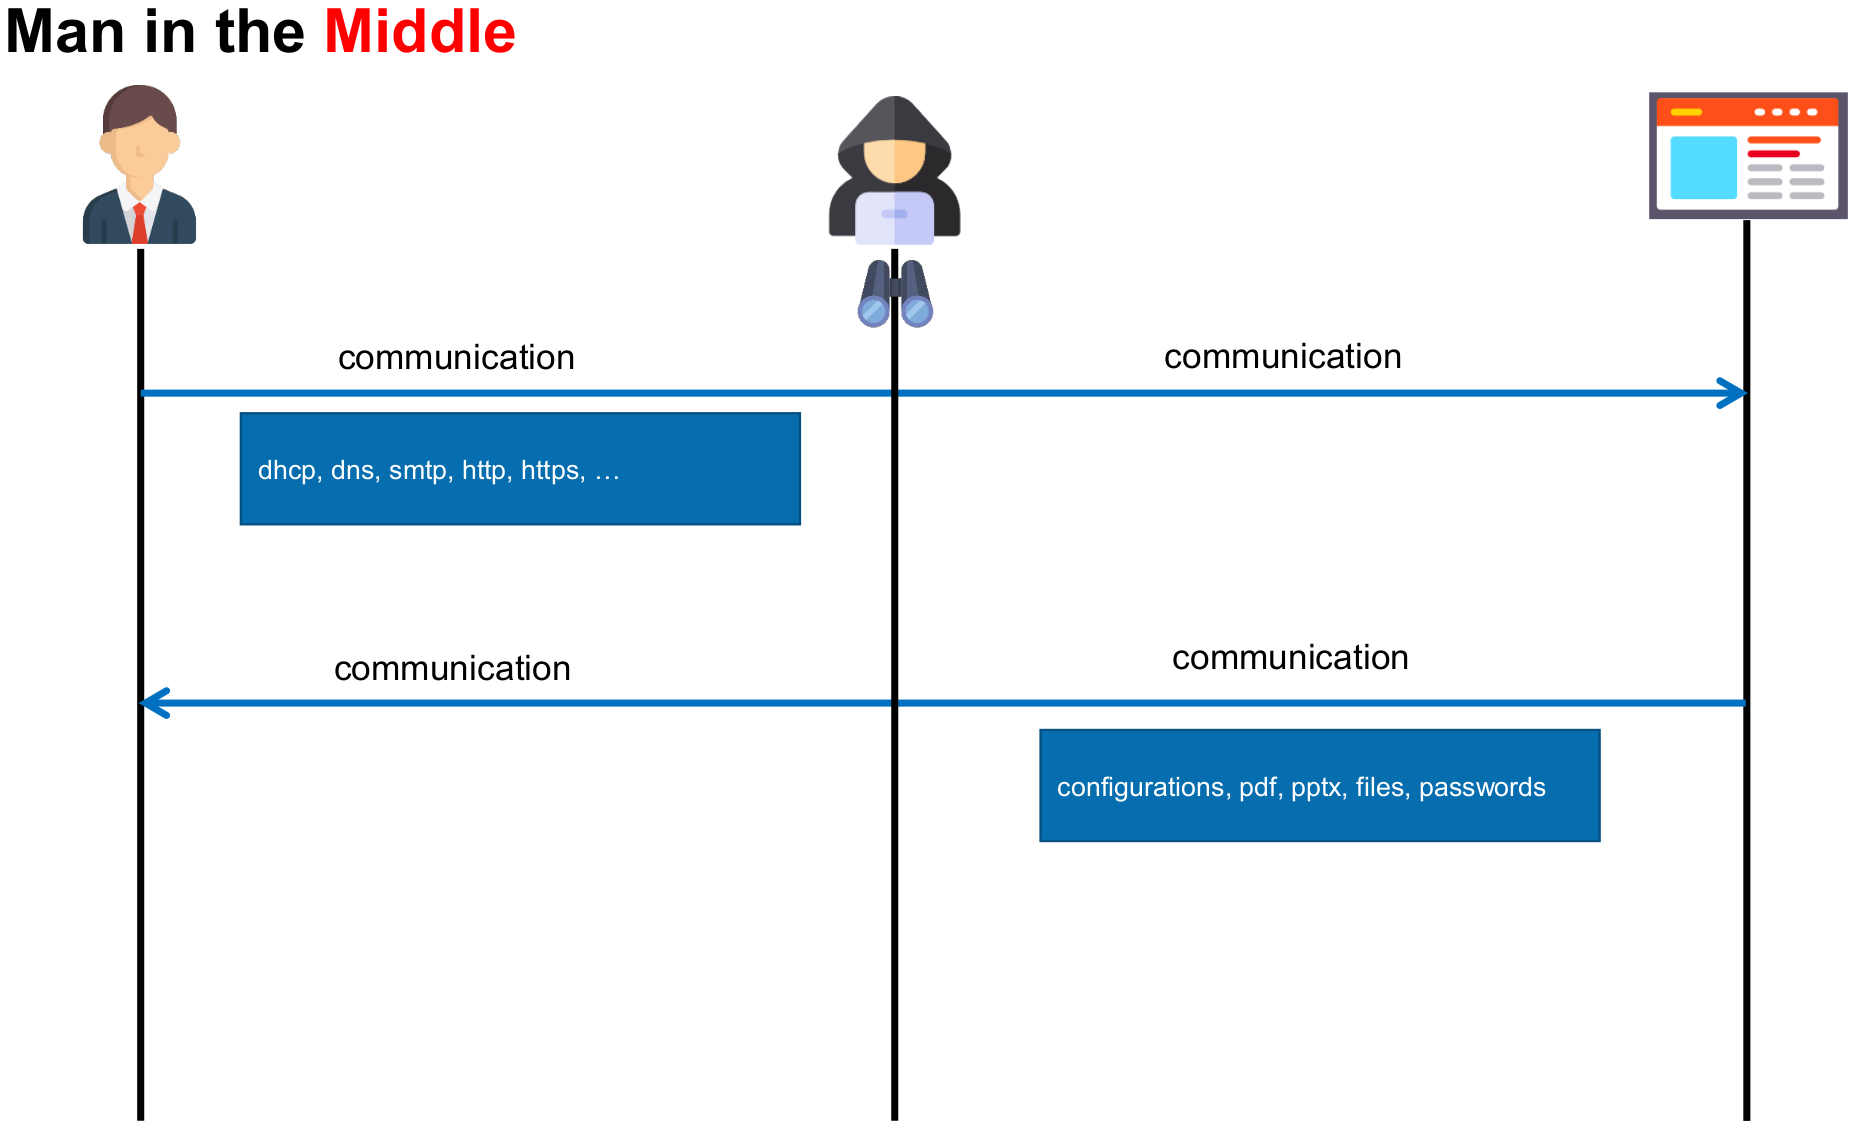
\includegraphics[width=\textwidth]{resources/07-mitm.png}
\end{center}
\textbf{Network Protocol Interception}
The MITM attacker can intercept and analyze:

\begin{itemize}
    \item \textbf{DHCP Traffic:}
        \begin{itemize}
            \item IP address assignments
            \item Network configuration parameters
            \item Default gateway information
        \end{itemize}
    
    \item \textbf{DNS Queries:}
        \begin{itemize}
            \item Domain name resolutions
            \item Website lookup patterns
            \item Opportunity for DNS spoofing
        \end{itemize}
        
    \item \textbf{HTTP/HTTPS:}
        \begin{itemize}
            \item Unencrypted HTTP content
            \item SSL/TLS handshakes
            \item Potential for SSL stripping attacks
            \item Web form submissions
            \item Cookie data
        \end{itemize}
        
    \item \textbf{SMTP:}
        \begin{itemize}
            \item Email contents
            \item Email metadata
            \item Attachments
        \end{itemize}
\end{itemize}

\textbf{Data Content Visibility}
The attacker can capture:

\begin{itemize}
    \item \textbf{Document Transfers:}
        \begin{itemize}
            \item PDF files
            \item PowerPoint presentations
            \item Word documents
            \item Spreadsheets
        \end{itemize}
    
    \item \textbf{Sensitive Information:}
        \begin{itemize}
            \item Login credentials
            \item Session tokens
            \item Authentication cookies
            \item Personal information
        \end{itemize}
        
    \item \textbf{Configuration Data:}
        \begin{itemize}
            \item System settings
            \item Network configurations
            \item Security parameters
        \end{itemize}
\end{itemize}

\textbf{Attack Capabilities}
\begin{itemize}
    \item \textbf{Active Manipulation:}
        \begin{itemize}
            \item Modify packet contents
            \item Inject malicious code
            \item Alter transaction details
            \item Redirect traffic
        \end{itemize}
    
    \item \textbf{Passive Monitoring:}
        \begin{itemize}
            \item Traffic analysis
            \item Data collection
            \item Behavioral profiling
            \item Credential harvesting
        \end{itemize}
\end{itemize}

\textbf{Mitigation Strategies}
To protect against MITM attacks:

\begin{itemize}
    \item Use strong encryption (TLS 1.3+)
    \item Implement certificate pinning
    \item Enable HSTS (HTTP Strict Transport Security)
    \item Use VPNs on untrusted networks
    \item Verify certificate validity
    \item Monitor for unusual network behavior
\end{itemize}

\subsubsection{Man in the Browser}
\begin{center}
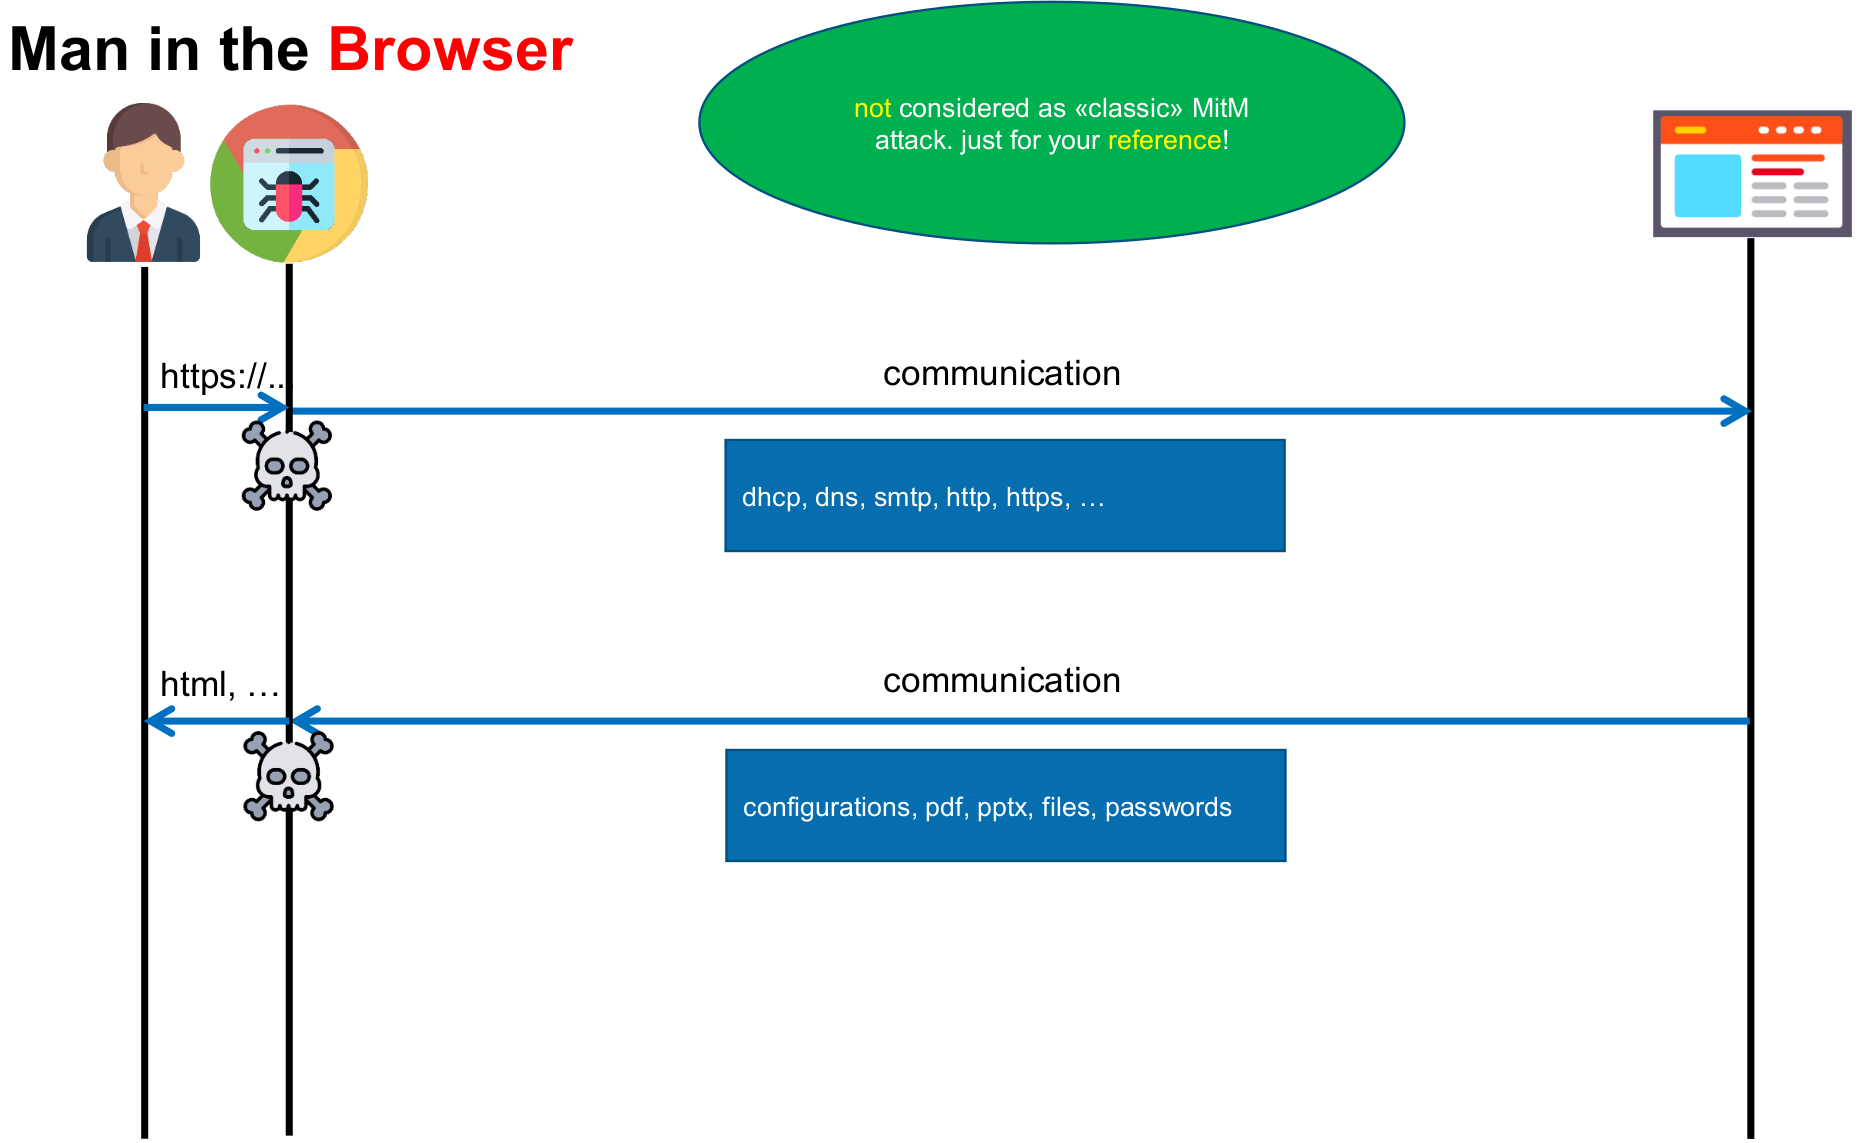
\includegraphics[width=\textwidth]{resources/07-mitb.png}
\end{center}
\textbf{Man-in-the-Browser Attack Overview}

A Man-in-the-Browser (MitB) attack operates by infecting the user's web browser with malware, typically through malicious extensions or trojans. Unlike MITM attacks that intercept network traffic, MitB malware integrates directly into the browser, allowing it to manipulate data in real-time before it's encrypted and sent to the server, or after it's received and decrypted. The image depicts this by showing the malware (represented by bug and skull icons) positioned directly at the browser level, with access to both incoming and outgoing communications.

\textbf{Protocols Involved}
\begin{itemize}
    \item HTTPS (primary target as MitB bypasses its encryption)
    \item HTTP (web traffic)
    \item HTML/JavaScript (for page manipulation)
    \item DOM (Document Object Model)
    \item Browser API protocols
    \item Form submission protocols
\end{itemize}

\textbf{Attack Capabilities}
\begin{itemize}
    \item Real-time web page content modification
    \item Form data interception before encryption
    \item JavaScript injection into legitimate pages
    \item Session hijacking
    \item Credential theft even with HTTPS
    \item Transaction manipulation while showing fake data to user
    \item Bypass of 2FA/MFA mechanisms
    \item Browser API manipulation
\end{itemize}

\textbf{Mitigation Strategies}
\begin{itemize}
    \item Regular browser security updates
    \item Extension vetting and minimal usage
    \item Endpoint Detection and Response (EDR) solutions
    \item Hardware security keys for authentication
    \item Out-of-band transaction verification
    \item Runtime application self-protection (RASP)
    \item Browser integrity checking
    \item Security-focused browser configurations
\end{itemize}

\subsubsection{MITM via BGP}
\begin{center}
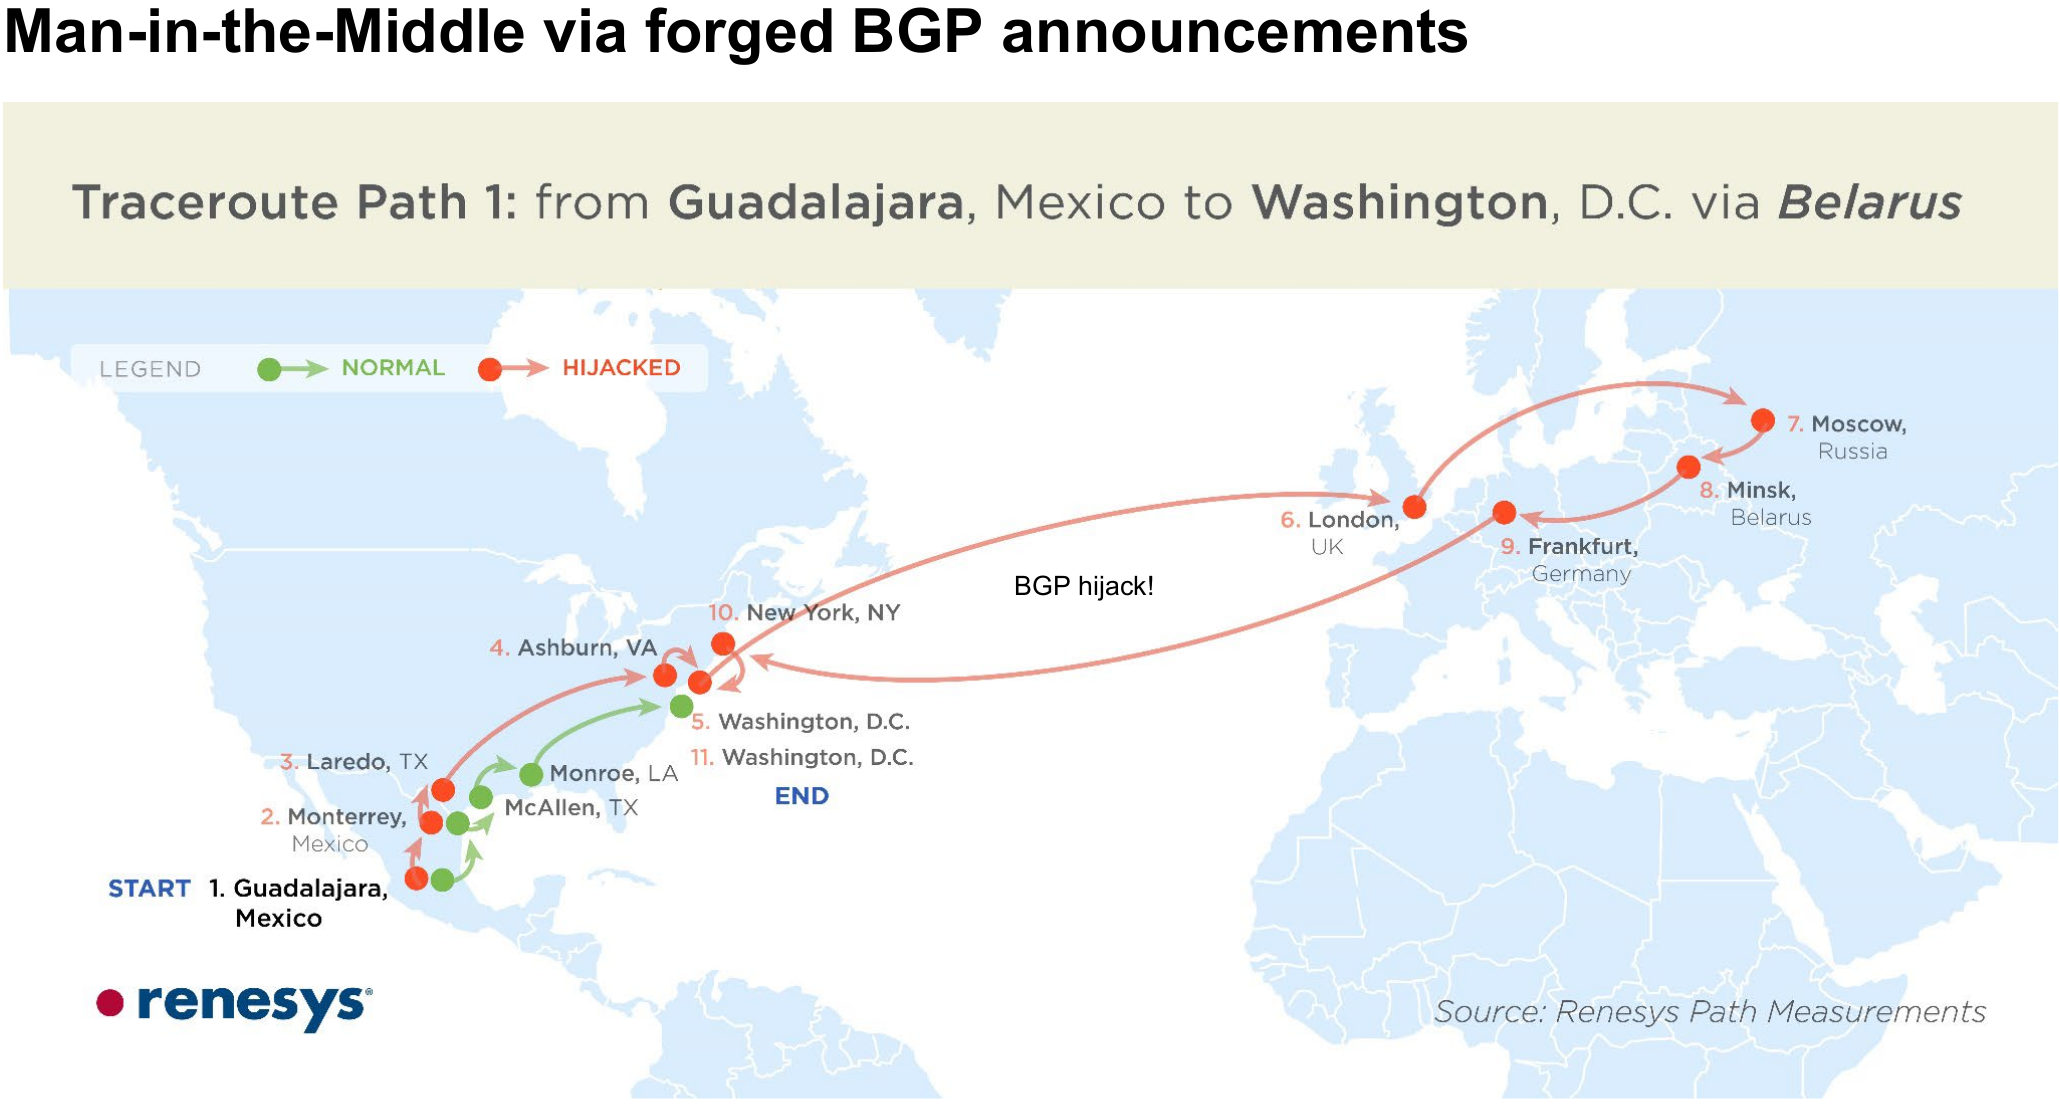
\includegraphics[width=\textwidth]{resources/07-mitm-via-bgp.png}
\end{center}
\textbf{BGP Hijacking Attack Overview}

This attack demonstrates a BGP (Border Gateway Protocol) hijacking scenario where the normal routing path from Guadalajara, Mexico to Washington D.C. is maliciously redirected through Belarus. The legitimate path (shown in green) routes through Texas and Louisiana, but the hijacked route (shown in red) forces traffic through multiple international points including New York, London, Moscow, Minsk, and Frankfurt. This type of attack exploits BGP's inherent trust model by announcing forged routes that claim to provide better paths to specific IP prefixes.

\textbf{Protocols Involved}
\begin{itemize}
    \item BGP (Border Gateway Protocol)
    \item TCP/IP
    \item AS (Autonomous System) protocols
    \item RPKI (Resource Public Key Infrastructure)
    \item BGP-SEC
\end{itemize}

\textbf{Attack Capabilities}
\begin{itemize}
    \item Traffic redirection through malicious nodes
    \item Interception of international data flows
    \item Creation of fake routing announcements
    \item AS path manipulation
    \item Route origin spoofing
    \item Prefix hijacking
    \item Route leak attacks
    \item Blackholing of traffic
\end{itemize}

\textbf{Mitigation Strategies}
\begin{itemize}
    \item Implementation of RPKI validation
    \item BGP route filtering
    \item Use of BGP-SEC when available
    \item Route origin authorization (ROA)
    \item Prefix filtering at internet exchanges
    \item Regular monitoring of BGP announcements
    \item Implementation of maximum prefix limits
    \item AS path verification
    \item IRR (Internet Routing Registry) filtering
\end{itemize}

\subsubsection{MTIM DHCP}
\begin{center}
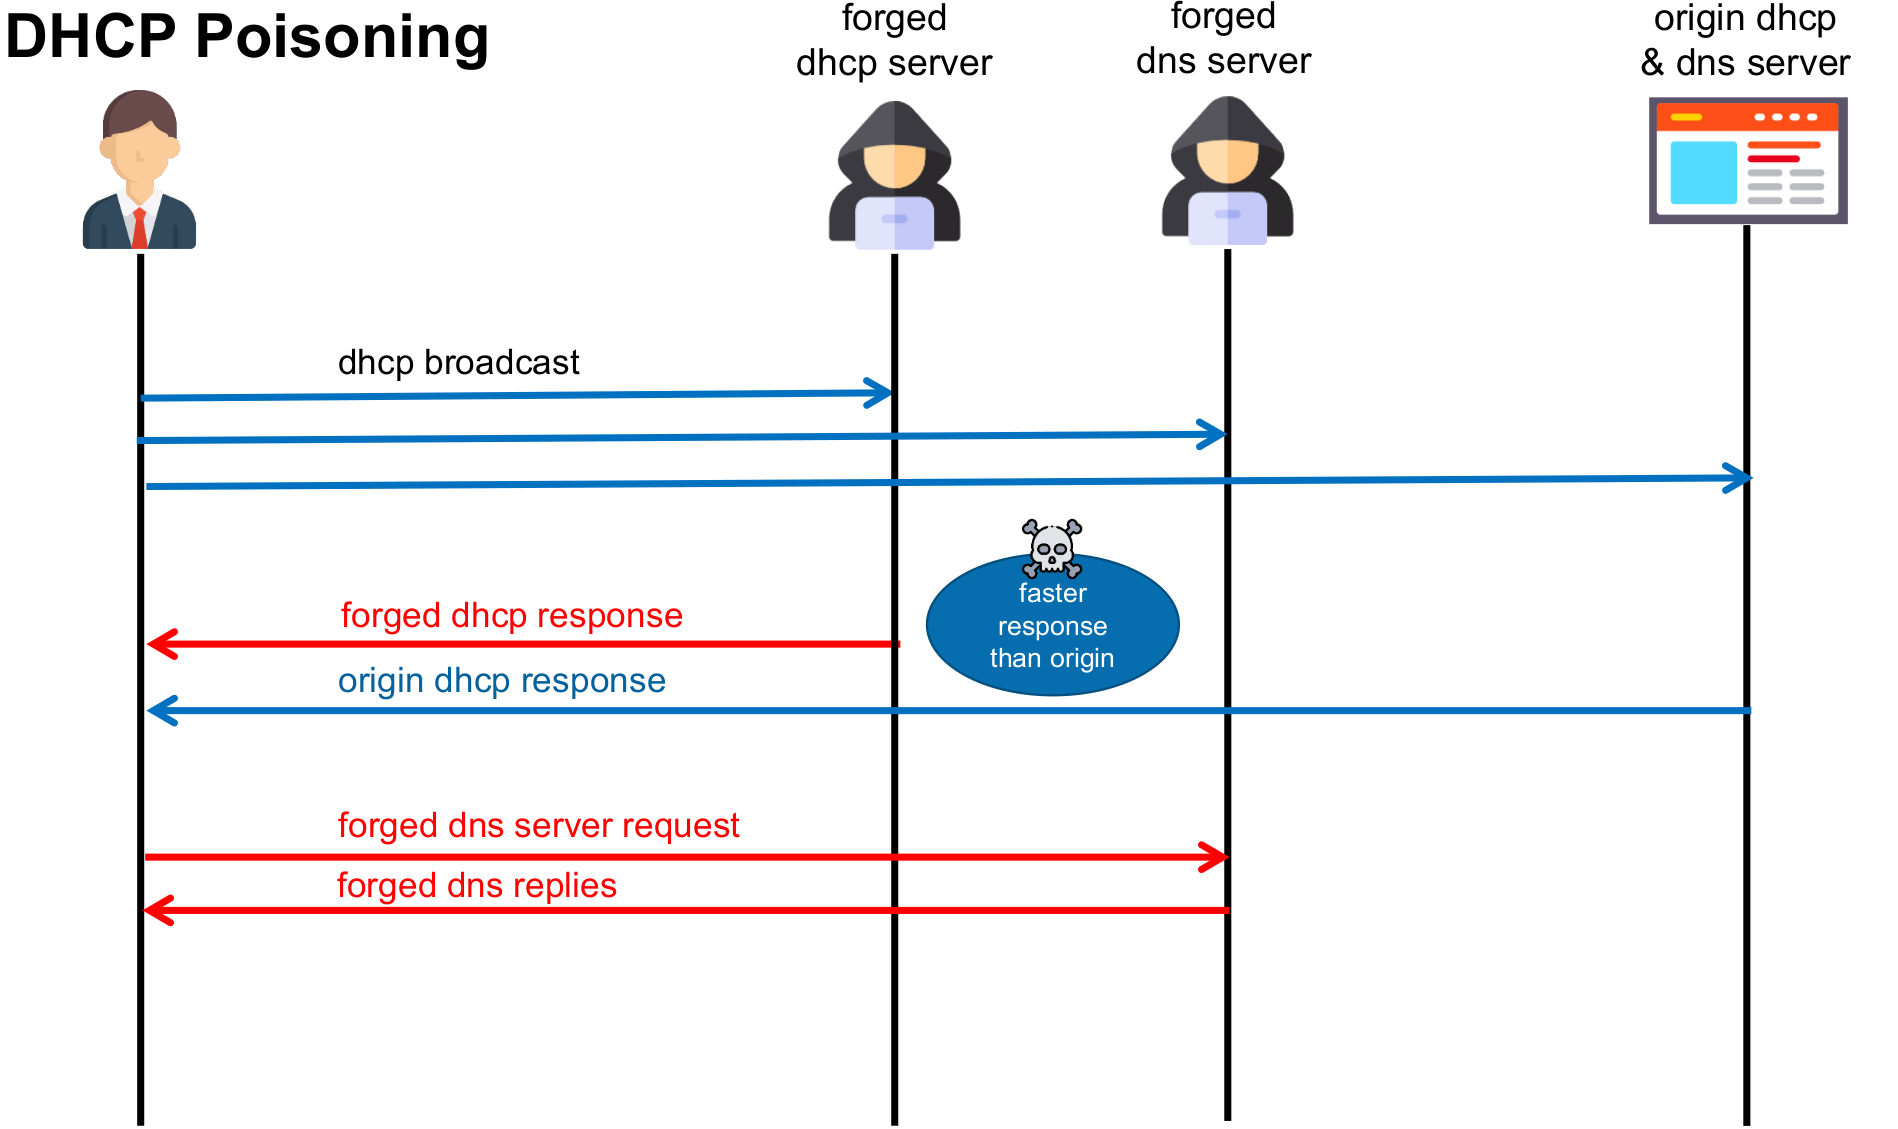
\includegraphics[width=\textwidth]{resources/07-dhcp-1.png}
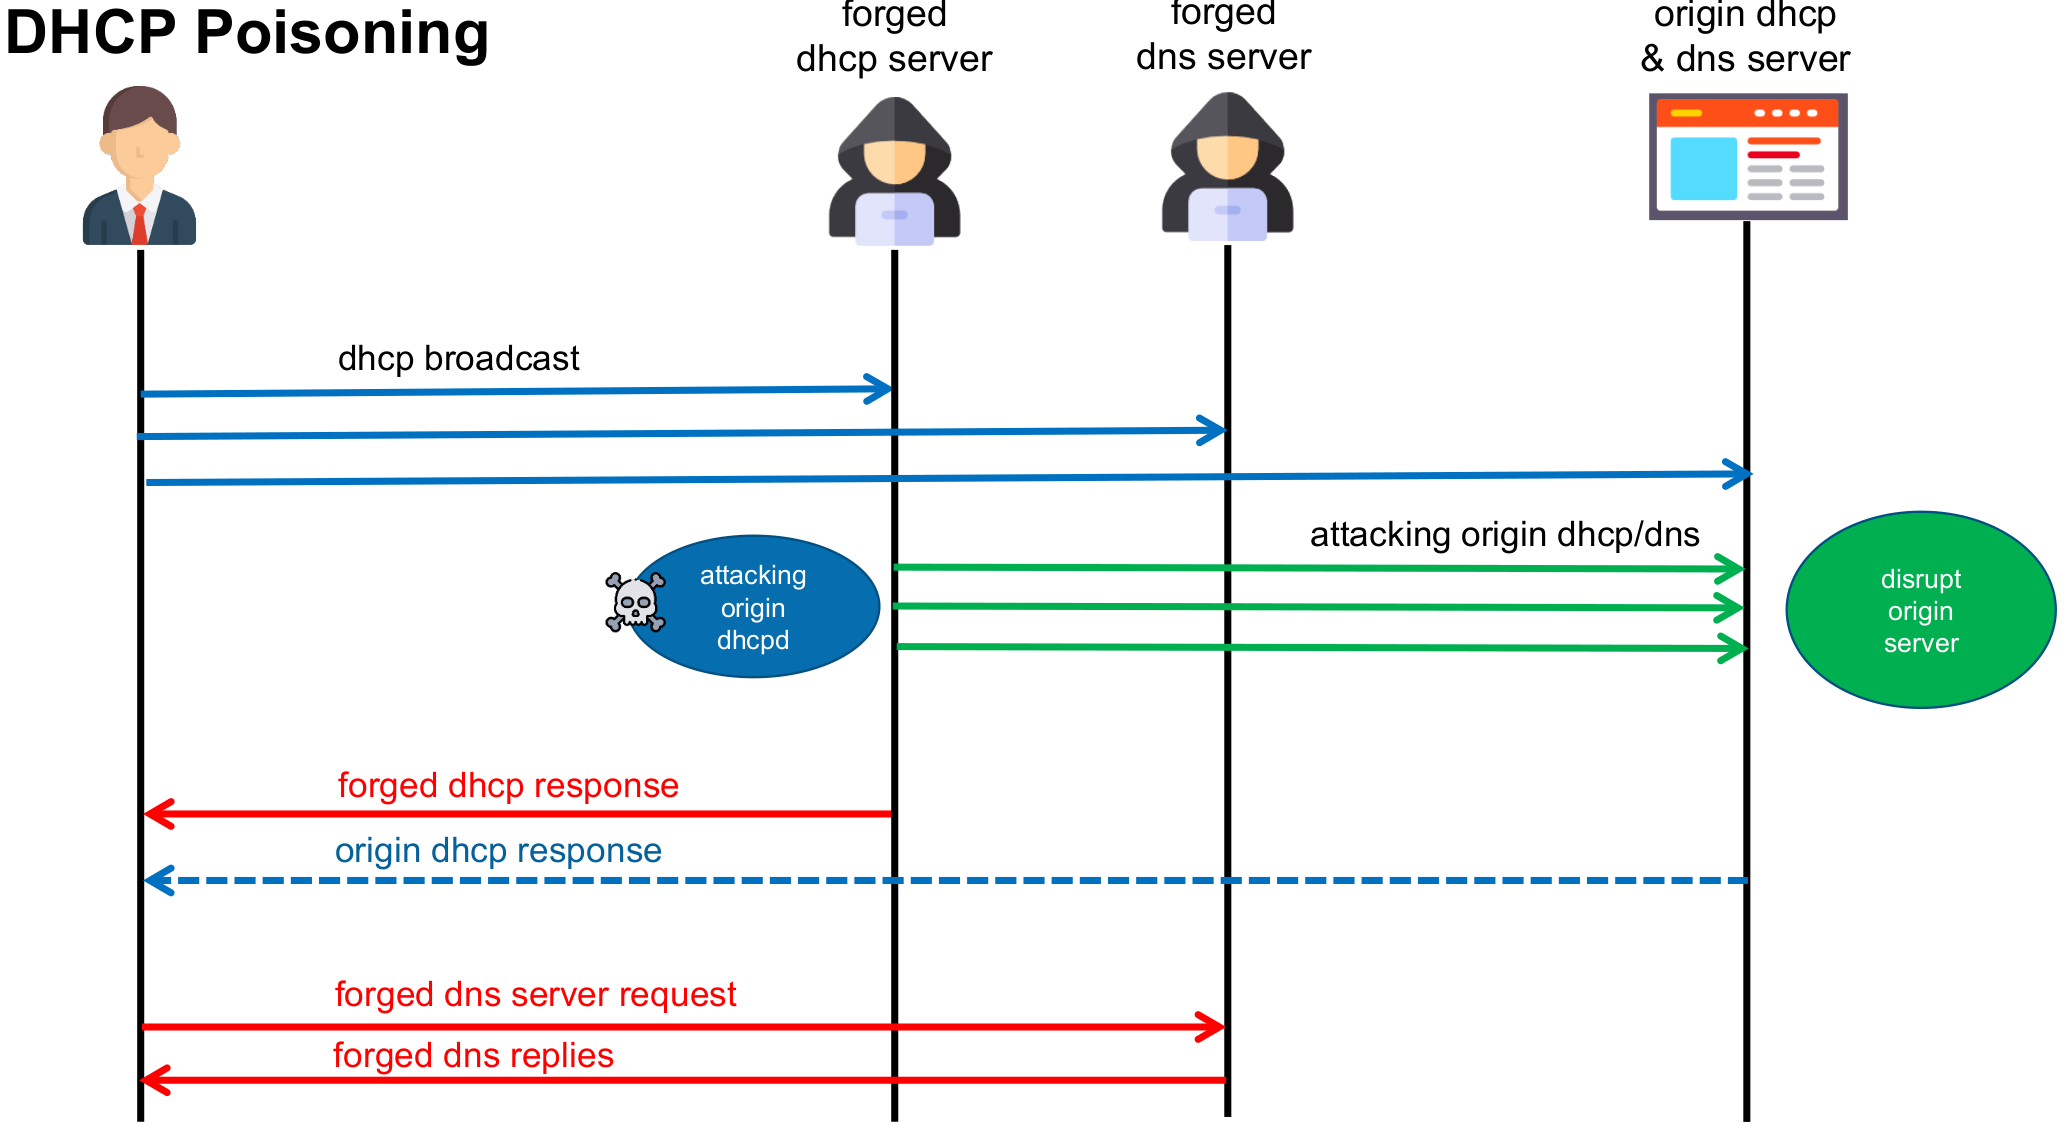
\includegraphics[width=\textwidth]{resources/07-dhcp-2.png}
\end{center}
\textbf{Attack Overview}

DHCP poisoning is illustrated here in two phases. In the first image, the attacker sets up rogue DHCP and DNS servers that respond faster than legitimate servers to intercept client requests. In the second image, the attack escalates to actively disrupting the original DHCP/DNS servers while maintaining control over client communications through the forged responses.

\textbf{Protocols Involved}
\begin{itemize}
    \item DHCP (Dynamic Host Configuration Protocol)
    \item DNS (Domain Name System)
    \item UDP/IP (underlying transport protocols)
    \item ARP (potentially used in combination)
    \item ICMP (for network discovery)
\end{itemize}

\textbf{Attack Capabilities}
\begin{itemize}
    \item Injection of malicious DHCP configurations
    \item DNS response manipulation
    \item Default gateway redirection
    \item Network parameters poisoning
    \item Service denial through DHCP exhaustion
    \item DNS cache poisoning
    \item Network topology mapping
    \item Traffic redirection to malicious servers
\end{itemize}

\textbf{Mitigation Strategies}
\begin{itemize}
    \item DHCP snooping implementation
    \item Dynamic ARP inspection
    \item Port security measures
    \item DHCP server authorization
    \item DNS Security Extensions (DNSSEC)
    \item Network access control
    \item DHCP authentication
    \item Server redundancy
    \item Regular network monitoring
    \item IPv6 RA Guard
\end{itemize}

\subsubsection{MITM dns Poisoning}
\begin{center}
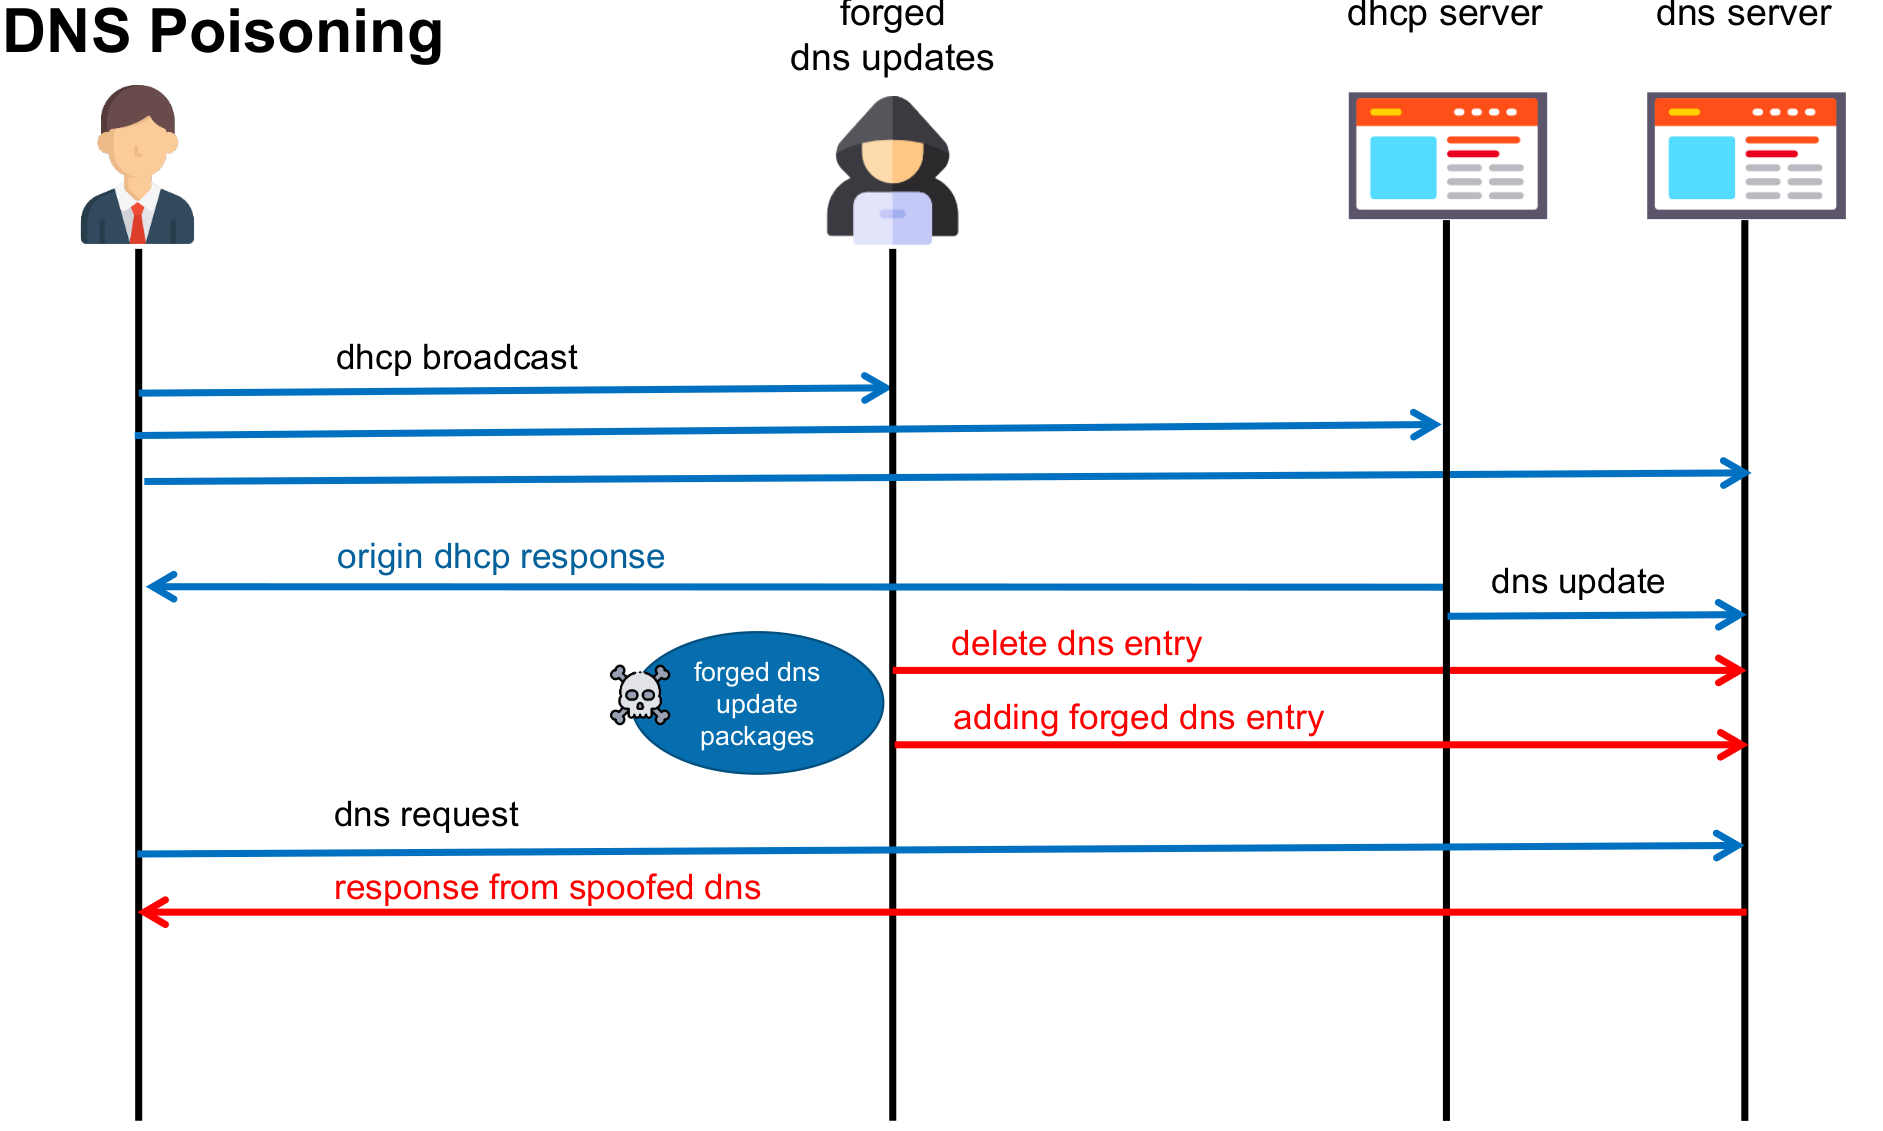
\includegraphics[width=\textwidth]{resources/07-dns-poisoning.png}
\end{center}
\textbf{Attack Overview}

DNS poisoning is demonstrated here where an attacker manipulates DNS entries through forged updates. The attack begins with normal DHCP operations, but the attacker then injects malicious DNS updates to delete legitimate DNS entries and replace them with forged ones. This results in the victim receiving spoofed DNS responses that redirect their traffic to potentially malicious destinations.

\textbf{Protocols Involved}
\begin{itemize}
    \item DNS (Domain Name System)
    \item DHCP (Dynamic Host Configuration Protocol)
    \item DNS Update Protocol (RFC 2136)
    \item TCP/UDP (transport protocols)
    \item IP (Internet Protocol)
\end{itemize}

\textbf{Attack Capabilities}
\begin{itemize}
    \item DNS cache manipulation
    \item Domain name resolution hijacking
    \item Website redirection
    \item DNS entry deletion
    \item Forged DNS record insertion
    \item DNS update packet forgery
    \item Man-in-the-middle positioning
    \item Phishing attack facilitation
\end{itemize}

\textbf{Mitigation Strategies}
\begin{itemize}
    \item DNSSEC implementation
    \item DNS update authentication
    \item Transaction signatures (TSIG)
    \item Access control lists (ACLs)
    \item DNS response validation
    \item Regular DNS audit logging
    \item Secure DNS update policies
    \item DNS server hardening
    \item DNS query monitoring
    \item Split DNS architecture
\end{itemize}

\subsubsection{MITM unencrypted}
\begin{center}
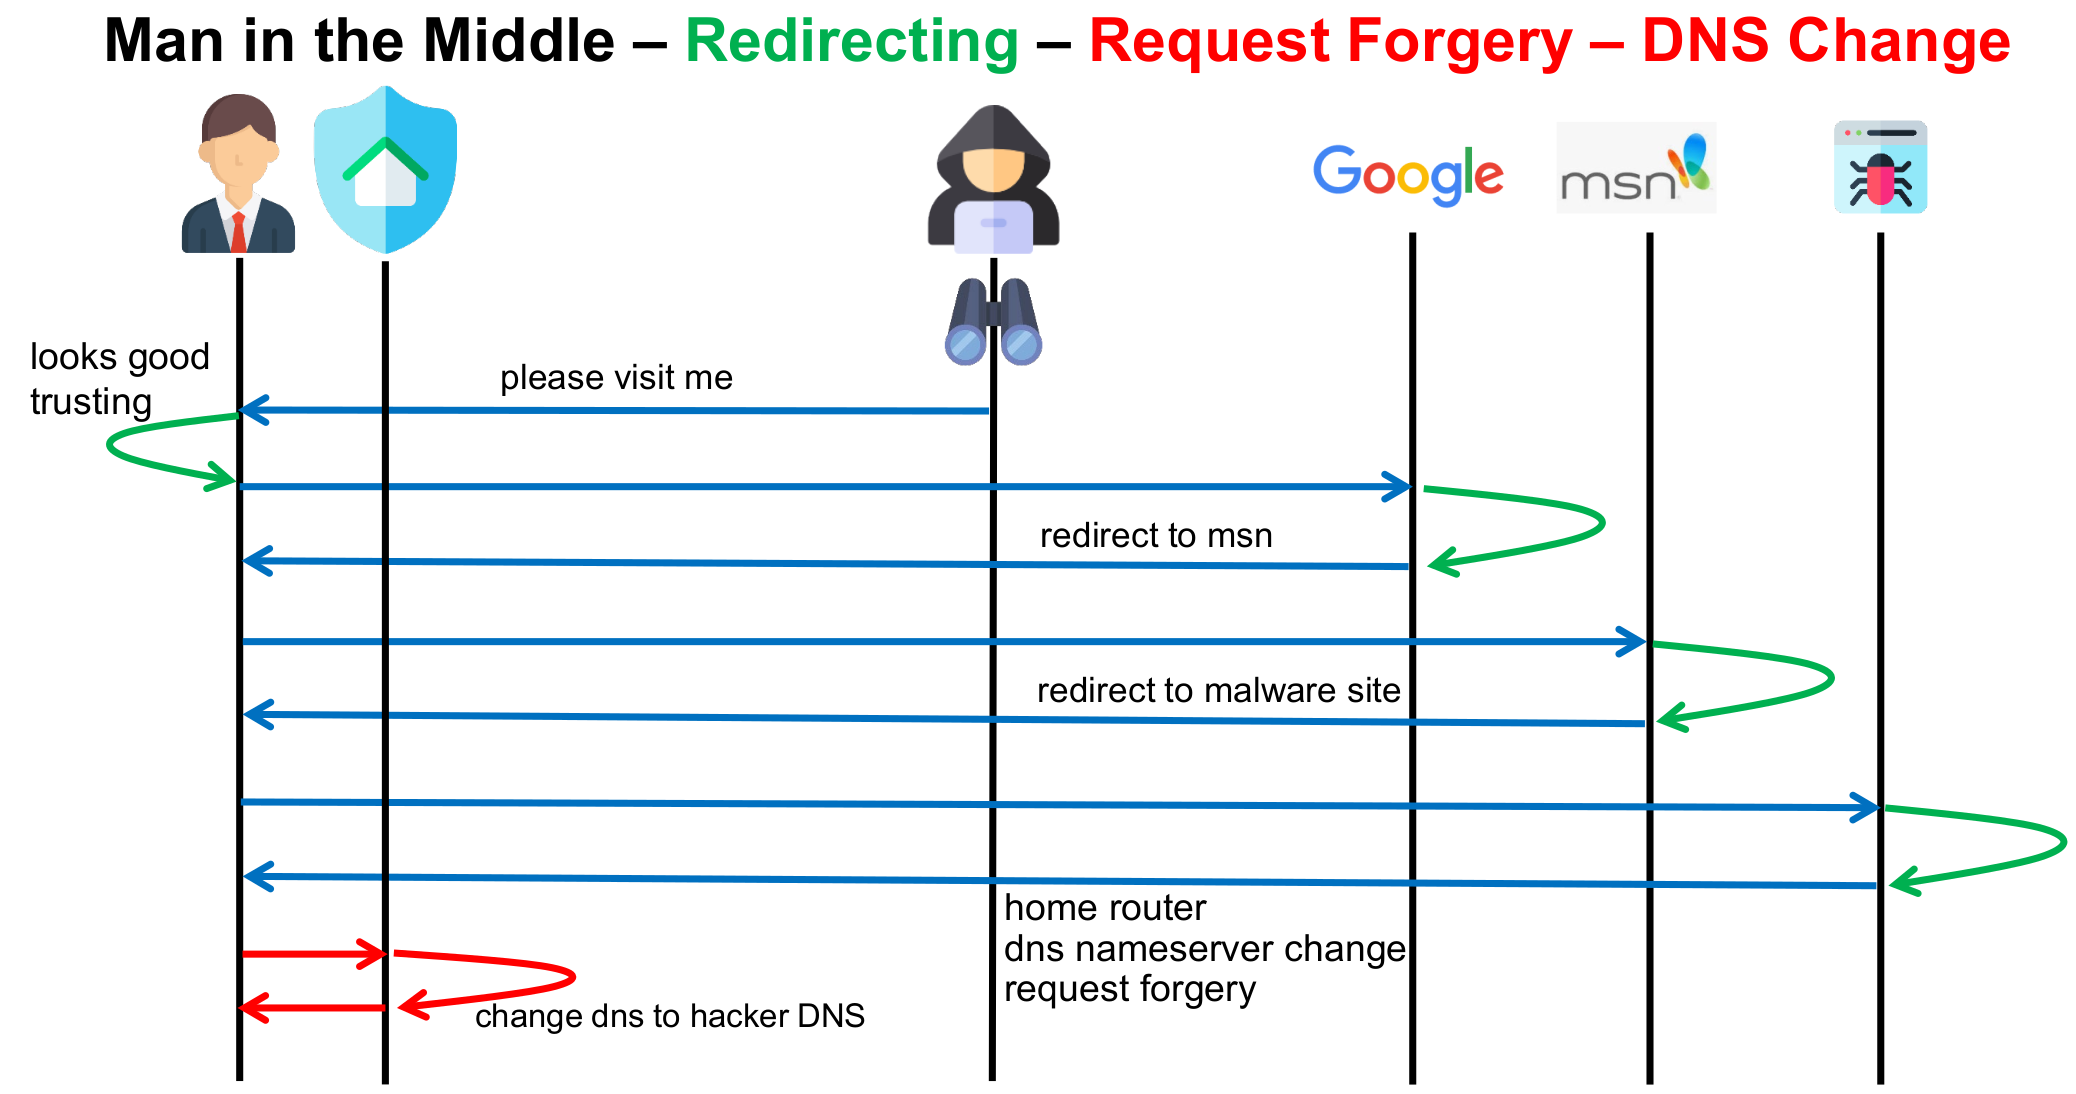
\includegraphics[width=\textwidth]{resources/07-mitm-request-forgery.png}
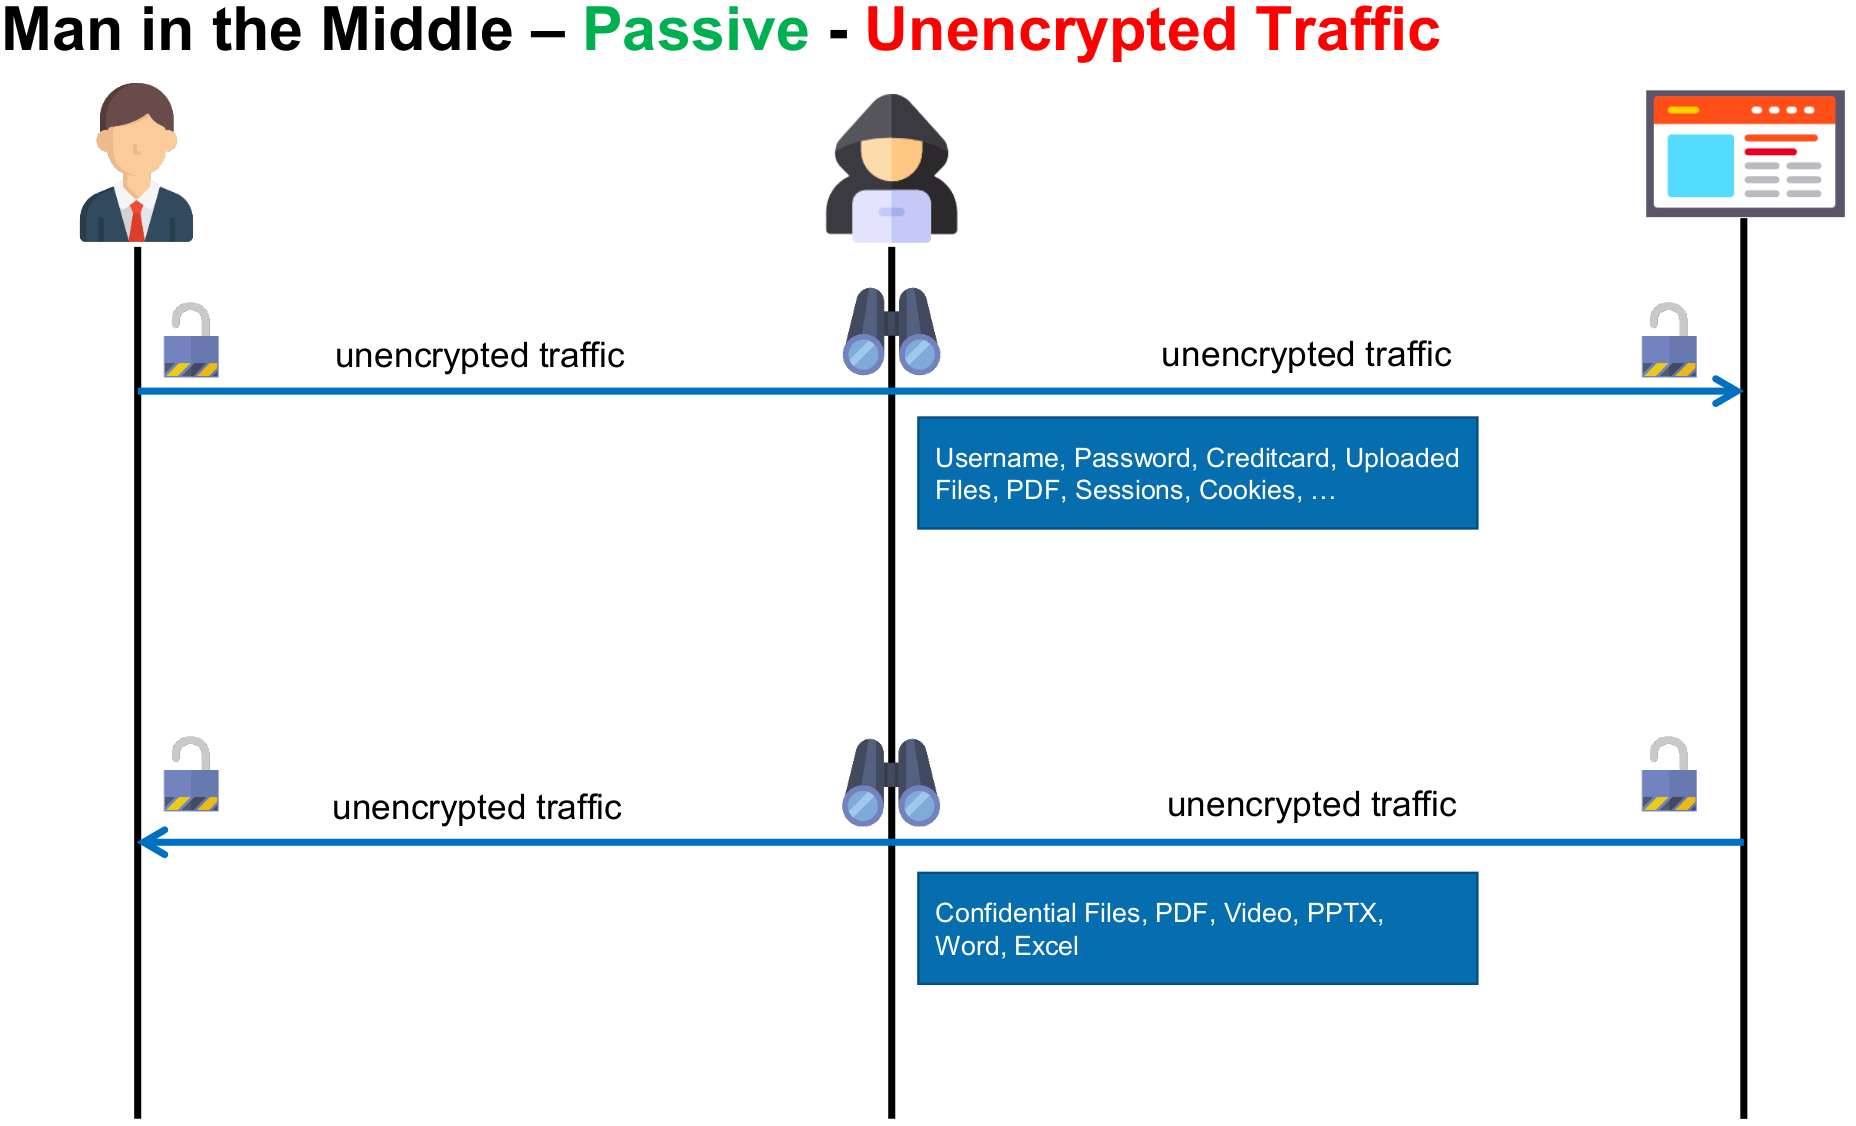
\includegraphics[width=\textwidth]{resources/07-mitm-passive-unencrypted.png}
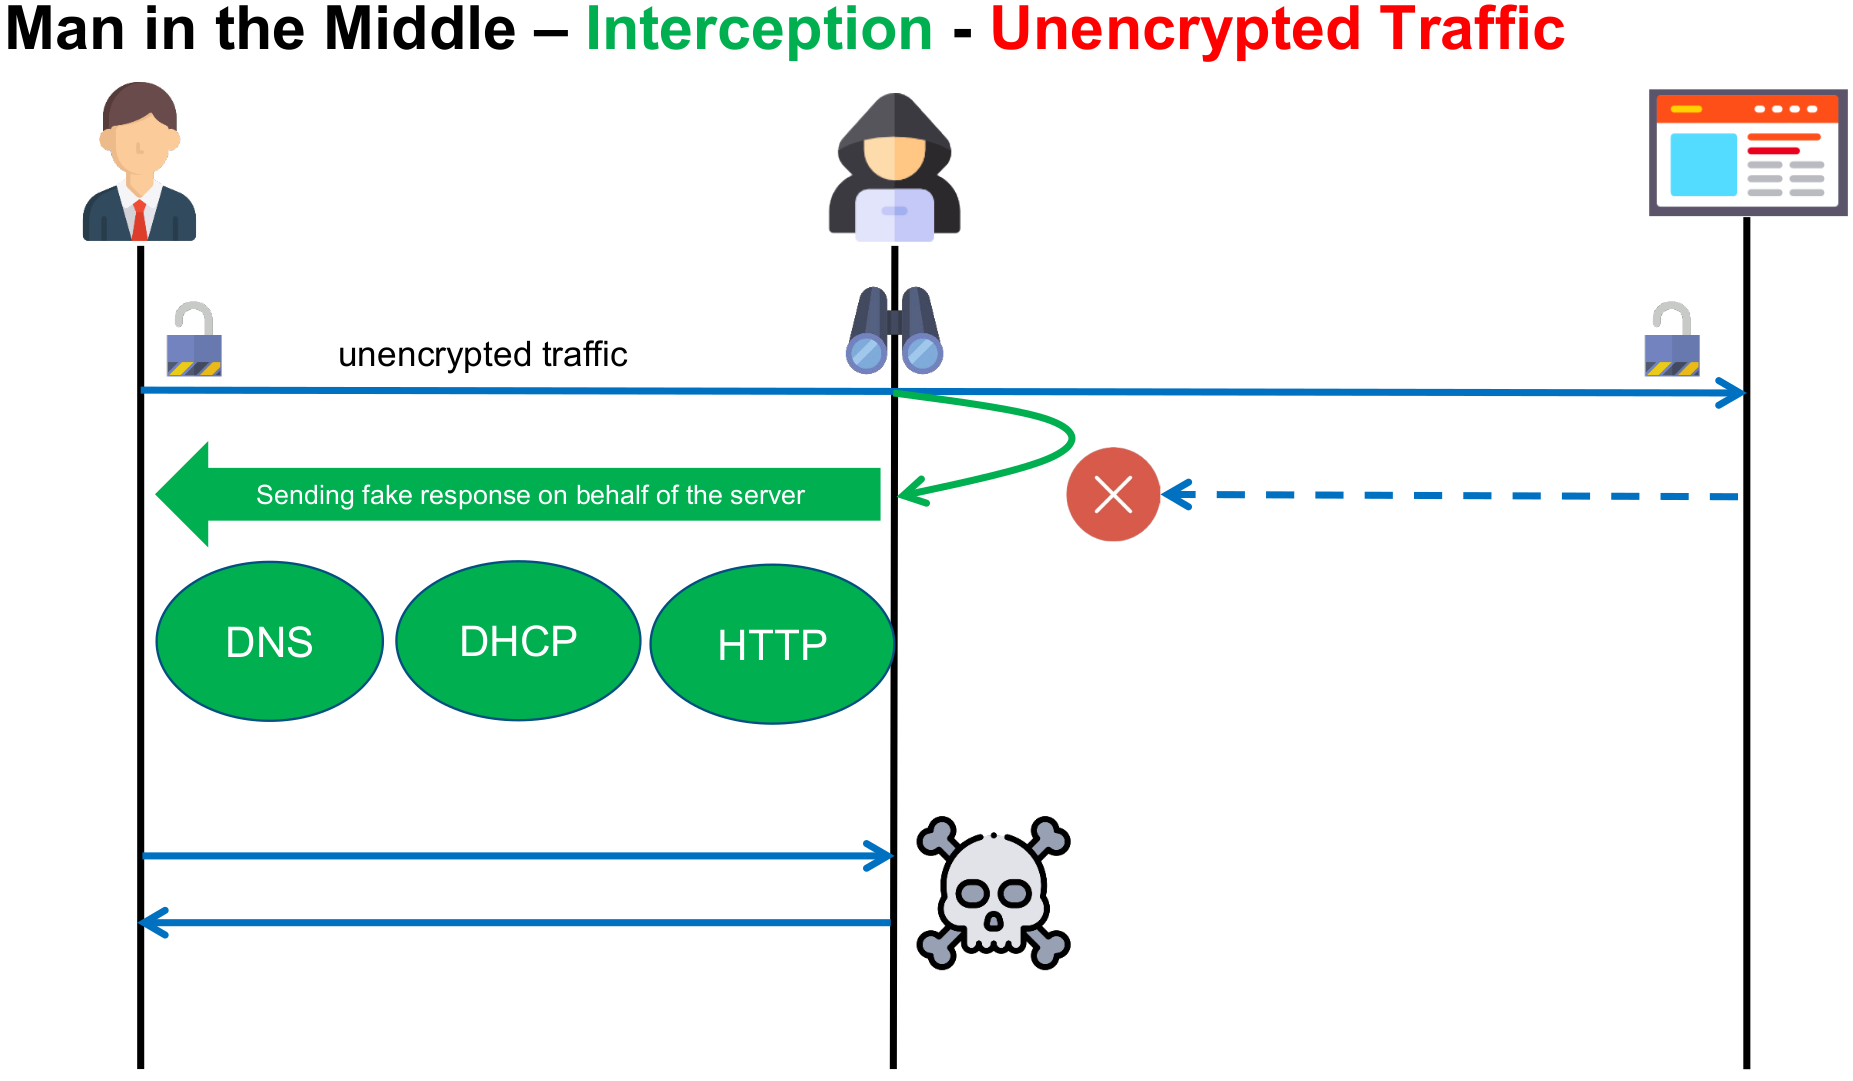
\includegraphics[width=\textwidth]{resources/07-mitm-passive-unencrypted-2.png}
\end{center}
\textbf{Attack Overview}

These images illustrate three stages of MITM attacks: passive monitoring of unencrypted traffic, active traffic redirection through DNS manipulation, and protocol interception. The first stage shows simple eavesdropping on unprotected data, the second demonstrates manipulation of traffic through DNS changes and request forgery, and the third shows active interception where the attacker blocks legitimate server responses while injecting fake ones.

\textbf{Protocols Involved}
\begin{itemize}
    \item HTTP (unencrypted web traffic)
    \item DNS (domain resolution)
    \item DHCP (network configuration)
    \item TCP/IP (transport and routing)
    \item TLS/SSL (when attempting to bypass)
    \item Router protocols (for home router manipulation)
\end{itemize}

\textbf{Attack Capabilities}
\begin{itemize}
    \item Passive traffic monitoring
    \item Credential harvesting
    \item Session hijacking
    \item Traffic redirection
    \item DNS manipulation
    \item Request forgery
    \item Response injection
    \item Home router reconfiguration
    \item Protocol downgrade attacks
    \item Malware distribution through redirects
\end{itemize}

\textbf{Mitigation Strategies}
\begin{itemize}
    \item Mandatory HTTPS implementation
    \item Certificate pinning
    \item DNS over HTTPS (DoH)
    \item HSTS enforcement
    \item Network segmentation
    \item Traffic encryption
    \item Regular security audits
    \item Network monitoring
    \item DNS security extensions (DNSSEC)
    \item Strong router configuration
\end{itemize}

\subsubsection{MITM encrypted}
\begin{center}
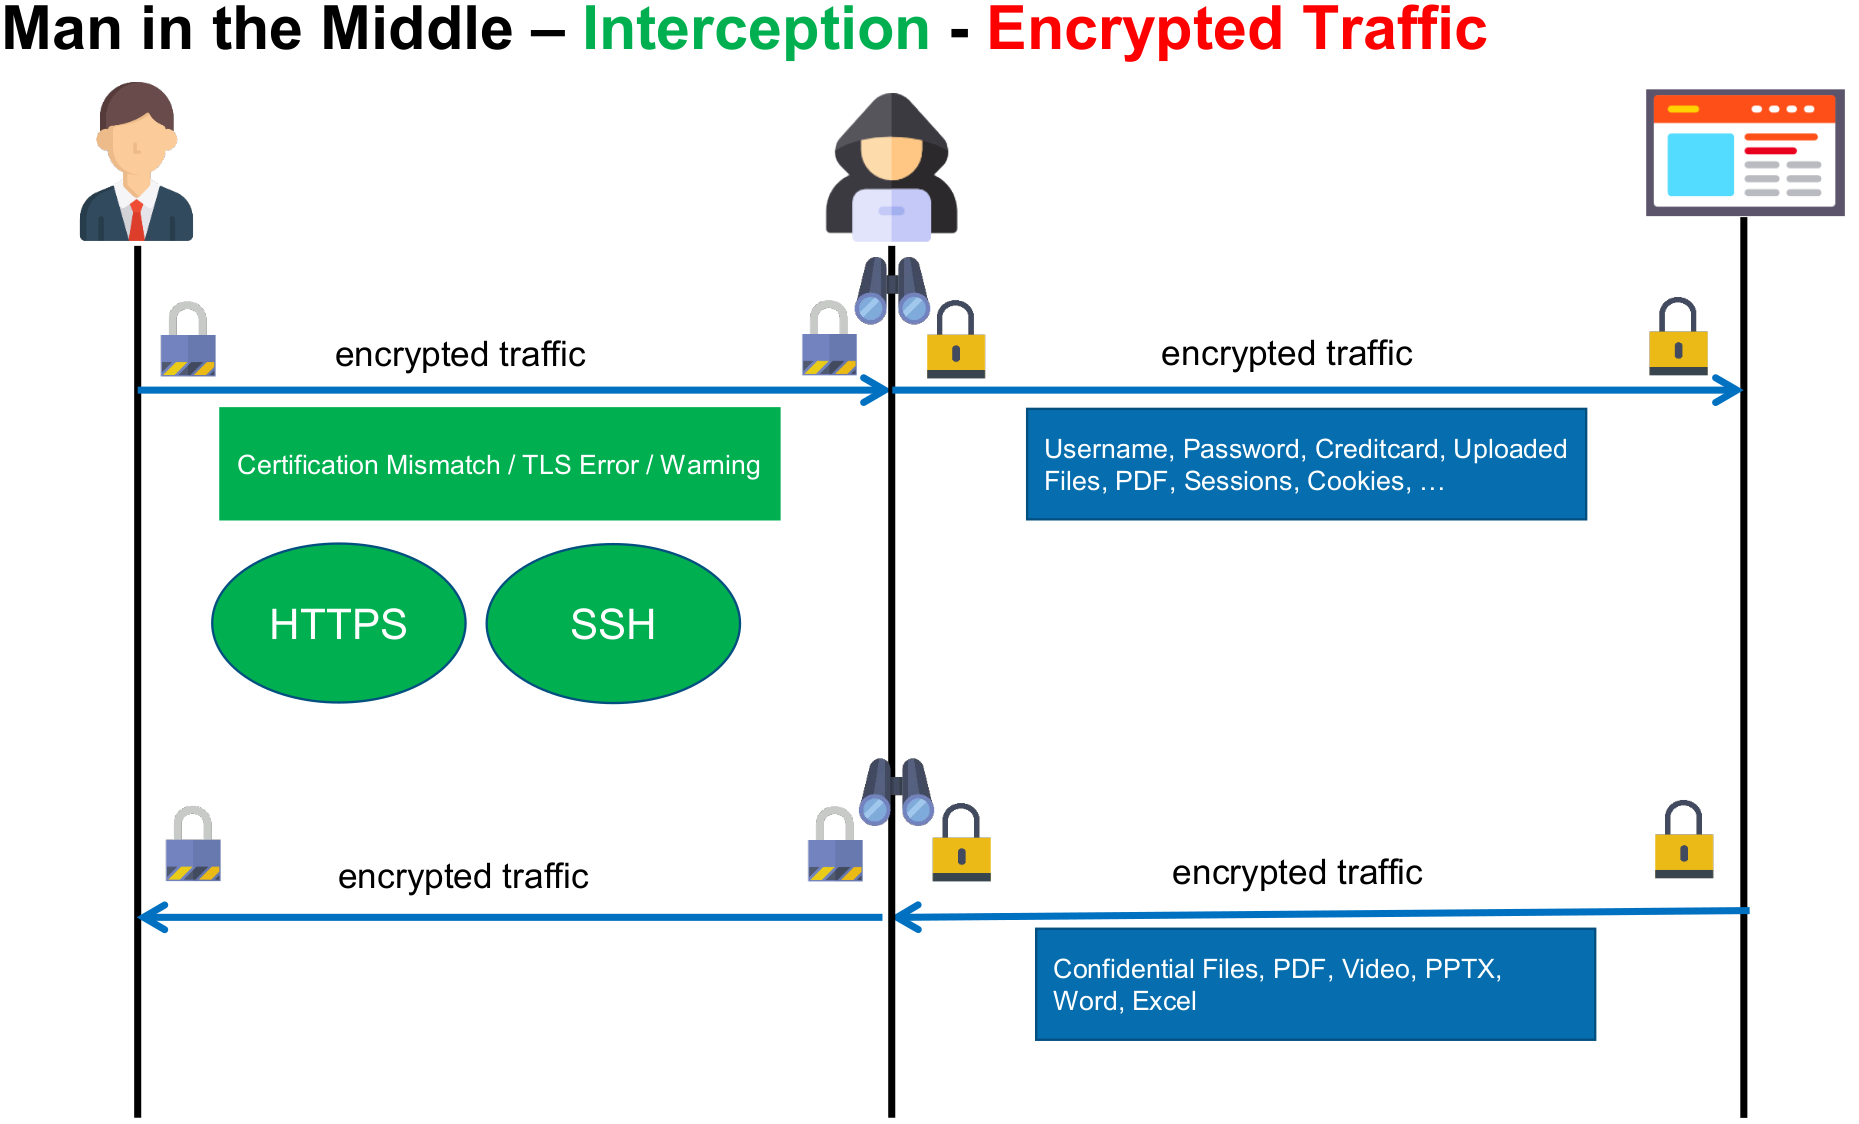
\includegraphics[width=\textwidth]{resources/07-mitm-interception-encrypted.png}
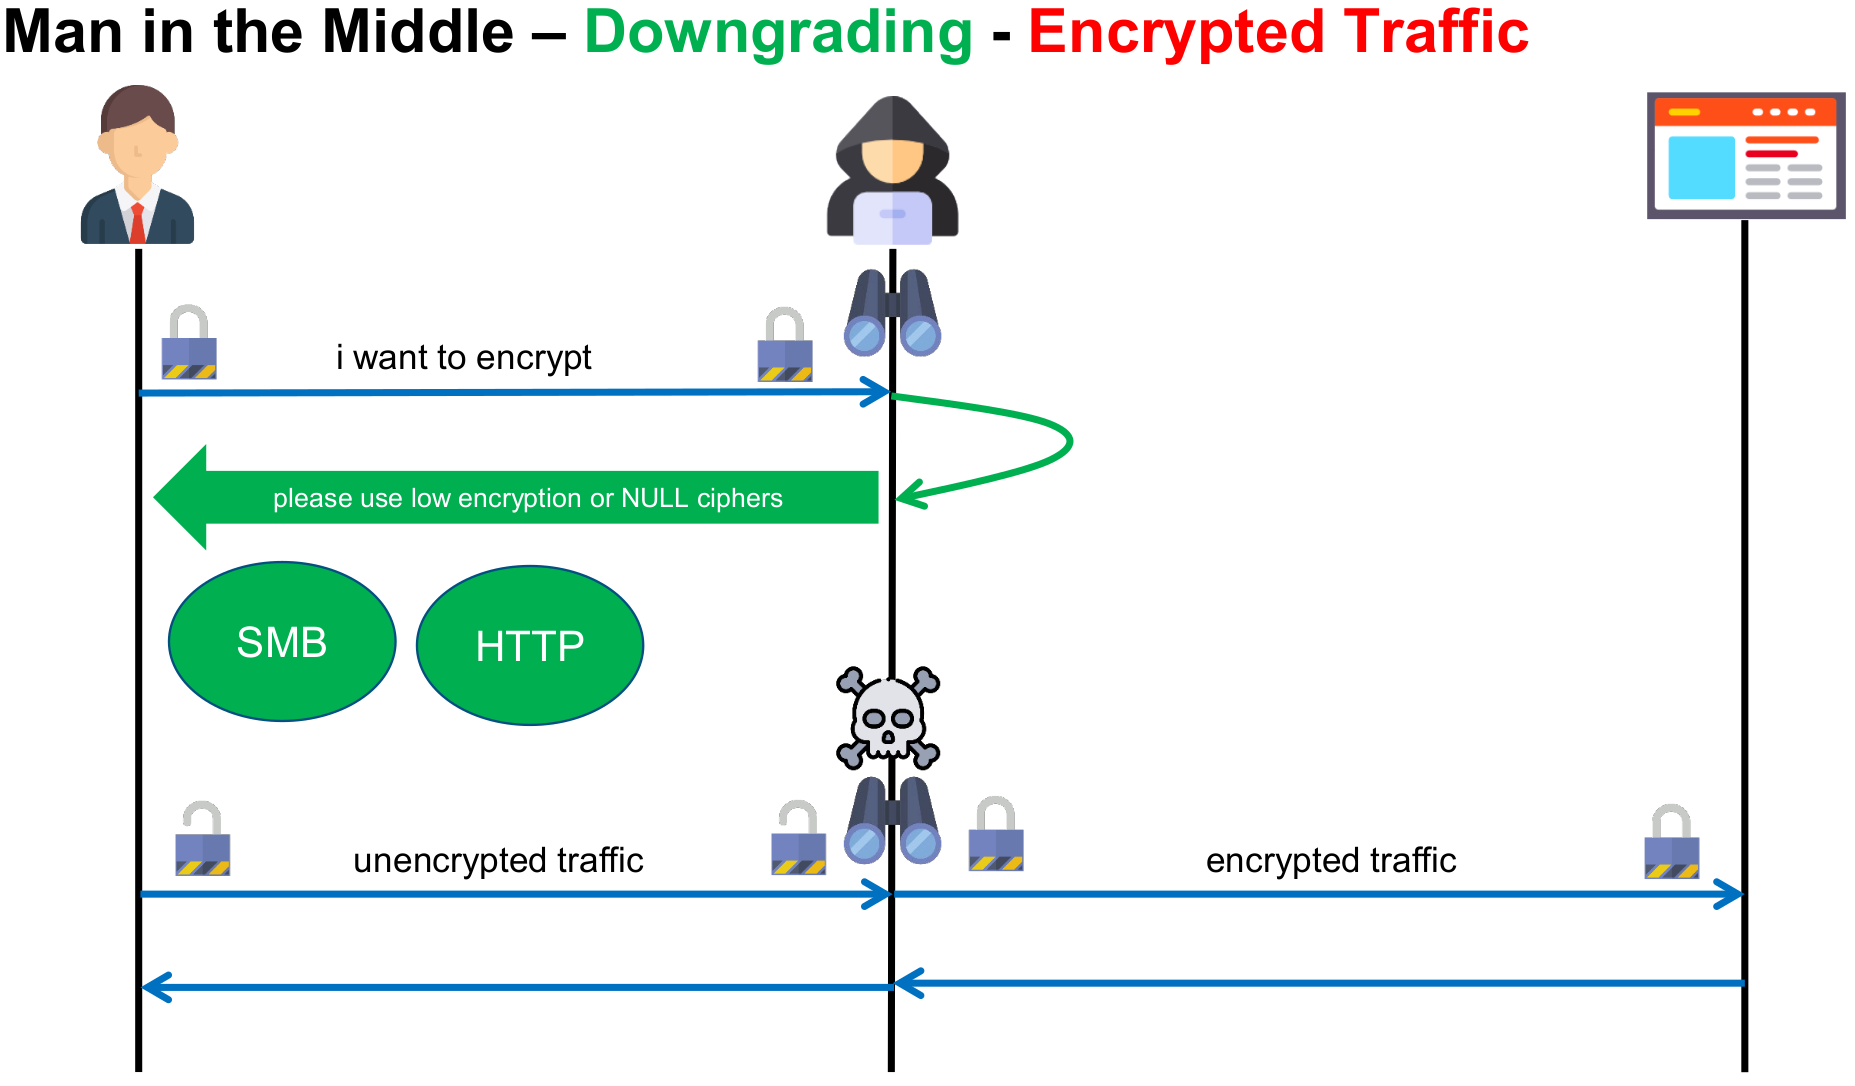
\includegraphics[width=\textwidth]{resources/07-mitm-interception-encrypted-1.png}
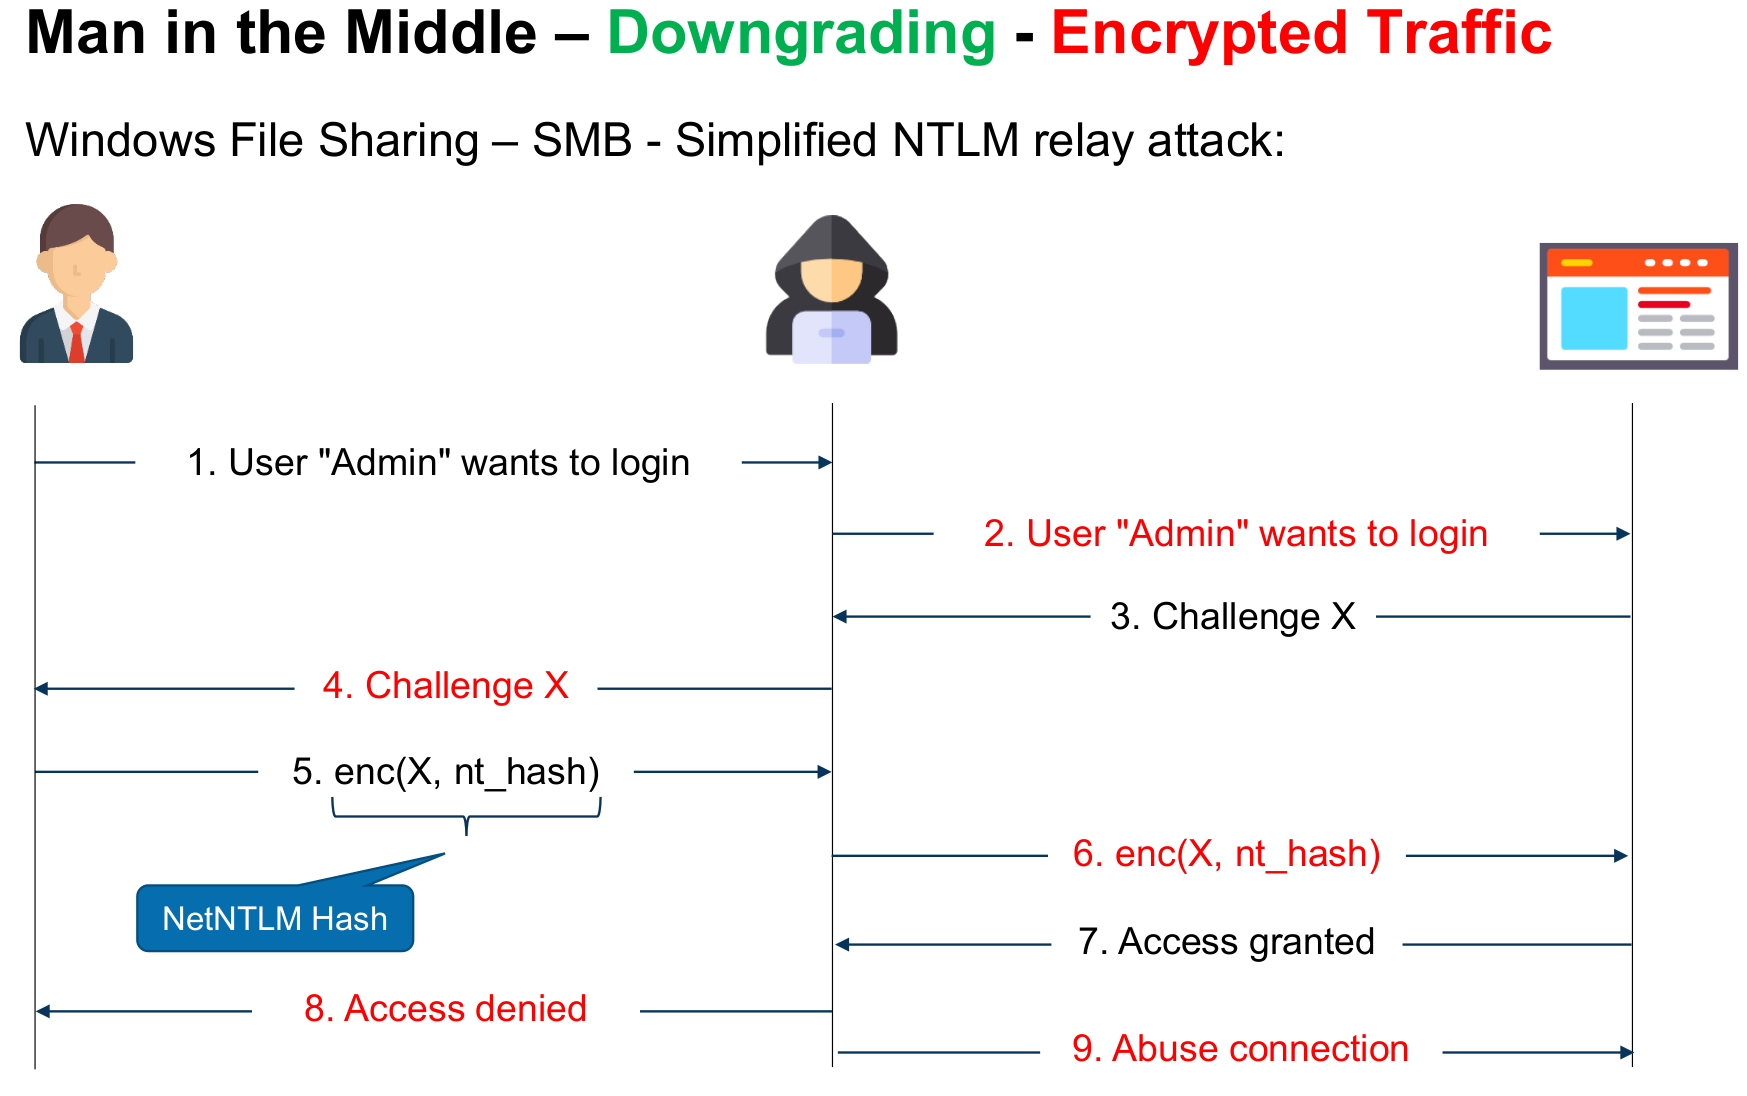
\includegraphics[width=\textwidth]{resources/07-mitm-interception-encrypted-2.png}
\end{center}
\textbf{Attack Overview}

These images demonstrate two sophisticated MITM attacks against encrypted traffic. The first shows an interception attack where the attacker attempts to break the encryption by exploiting certificate/TLS vulnerabilities, while the second illustrates a downgrade attack that forces the use of weaker encryption or no encryption at all. In both cases, the attacker tries to bypass the protection that encrypted protocols like HTTPS and SSH typically provide.

\textbf{Protocols Involved}
\begin{itemize}
    \item HTTPS (encrypted web traffic)
    \item SSH (secure shell)
    \item TLS/SSL (transport layer security)
    \item SMB (server message block)
    \item Certificate protocols
    \item TCP/IP (underlying transport)
\end{itemize}

\textbf{Attack Capabilities}
\begin{itemize}
    \item SSL/TLS interception
    \item Protocol downgrade attacks
    \item Certificate manipulation
    \item Cipher suite downgrade
    \item Forced weak encryption
    \item NULL cipher exploitation
    \item Session hijacking
    \item Credential harvesting
    \item Certificate spoofing
    \item Encryption stripping
\end{itemize}

\textbf{Mitigation Strategies}
\begin{itemize}
    \item Strict TLS version enforcement
    \item Certificate pinning implementation
    \item HSTS (HTTP Strict Transport Security)
    \item Strong cipher suite policies
    \item Regular certificate validation
    \item Security header implementation
    \item TLS 1.3+ requirement
    \item Certificate Authority verification
    \item SSL/TLS monitoring
    \item Security awareness training
\end{itemize}


\subsection{MITM HTTPS - Offline Phishing}
\begin{itemize}
    \item Fake https page: sent via e-mail
    \item Homograph Attack (cnsc instead of csnc) -> see DNSTwist
\end{itemize}

\subsubsection*{Mitigation}
\textbf{Fake HTTPS Pages in Phishing Emails}
\begin{itemize}
\item Email filtering and scanning systems
\item SSL/TLS certificate verification
\item Anti-phishing browser extensions
\item DMARC, SPF, and DKIM implementation
\item User security awareness training on:
\begin{itemize}
\item Checking full URLs before clicking
\item Verifying certificate validity
\item Not trusting unsolicited emails
\item Manual URL entry for sensitive sites
\end{itemize}
\item Implementing phishing reporting systems
\item Multi-factor authentication (MFA)
\end{itemize}
\textbf{Homograph Attacks (using DNSTwist-like techniques)}
\begin{itemize}
\item Technical Controls:
\begin{itemize}
\item IDN (Internationalized Domain Name) filtering
\item Domain monitoring services
\item DNS security solutions
\item Punycode enforcement in browsers
\item Regular domain typosquatting scans
\end{itemize}
\item Defensive Registration:
\begin{itemize}
\item Register common misspellings
\item Register similar-looking domains
\item Register Unicode variants
\item Protect all TLD variations
\end{itemize}
\item Active Monitoring:
\begin{itemize}
\item Use DNSTwist-like tools proactively
\item Monitor certificate issuance
\item Track domain registration patterns
\item Set up alerts for similar domains
\end{itemize}
\end{itemize}
\textbf{General Organizational Measures}
\begin{itemize}
\item Regular security assessments
\item Incident response planning
\item User training programs
\item Domain monitoring services
\item Certificate transparency monitoring
\item Brand protection services
\item Web filtering solutions
\item Regular penetration testing
\end{itemize}

\subsection{MITM HTTPS - Online Phishing}
\begin{itemize}
    \item https2hhtps
    \item http2hhtps
\end{itemize}
\textbf{Prevention Techniques for HTTPS MITM Phishing}

\begin{itemize}
    \item \textbf{Server-Side Controls}
        \begin{itemize}
            \item Implement HSTS (HTTP Strict Transport Security)
            \item Enable HSTS Preloading
            \item Deploy CAA (Certificate Authority Authorization)
            \item Use TLS 1.3 exclusively
            \item Implement proper SSL/TLS configuration
            \item Certificate pinning implementation
        \end{itemize}
    
    \item \textbf{Infrastructure Controls}
        \begin{itemize}
            \item Deploy DNSSEC
            \item Implement DNS over HTTPS (DoH)
            \item Use Extended Validation (EV) certificates
            \item Monitor Certificate Transparency logs
            \item Implement proper Content Security Policy (CSP)
            \item Enable automatic HTTPS redirects
        \end{itemize}

    \item \textbf{Client-Side Controls}
        \begin{itemize}
            \item Browser-enforced HTTPS
            \item Certificate validation
            \item TLS inspection
            \item URL filtering
            \item Secure browser configurations
            \item Anti-phishing browser extensions
        \end{itemize}
\end{itemize}

\textbf{Mitigation Strategies}
\begin{itemize}
    \item \textbf{Real-time Detection}
        \begin{itemize}
            \item SSL/TLS monitoring
            \item Network traffic analysis
            \item Certificate chain validation
            \item Protocol anomaly detection
            \item Real-time URL scanning
        \end{itemize}
    
    \item \textbf{Response Actions}
        \begin{itemize}
            \item Rapid incident response
            \item Certificate revocation
            \item Block malicious domains
            \item User notification systems
            \item Traffic redirection to legitimate sites
        \end{itemize}
\end{itemize}

\subsubsection{Online Phishing}
\textbf{http2https}
\begin{center}
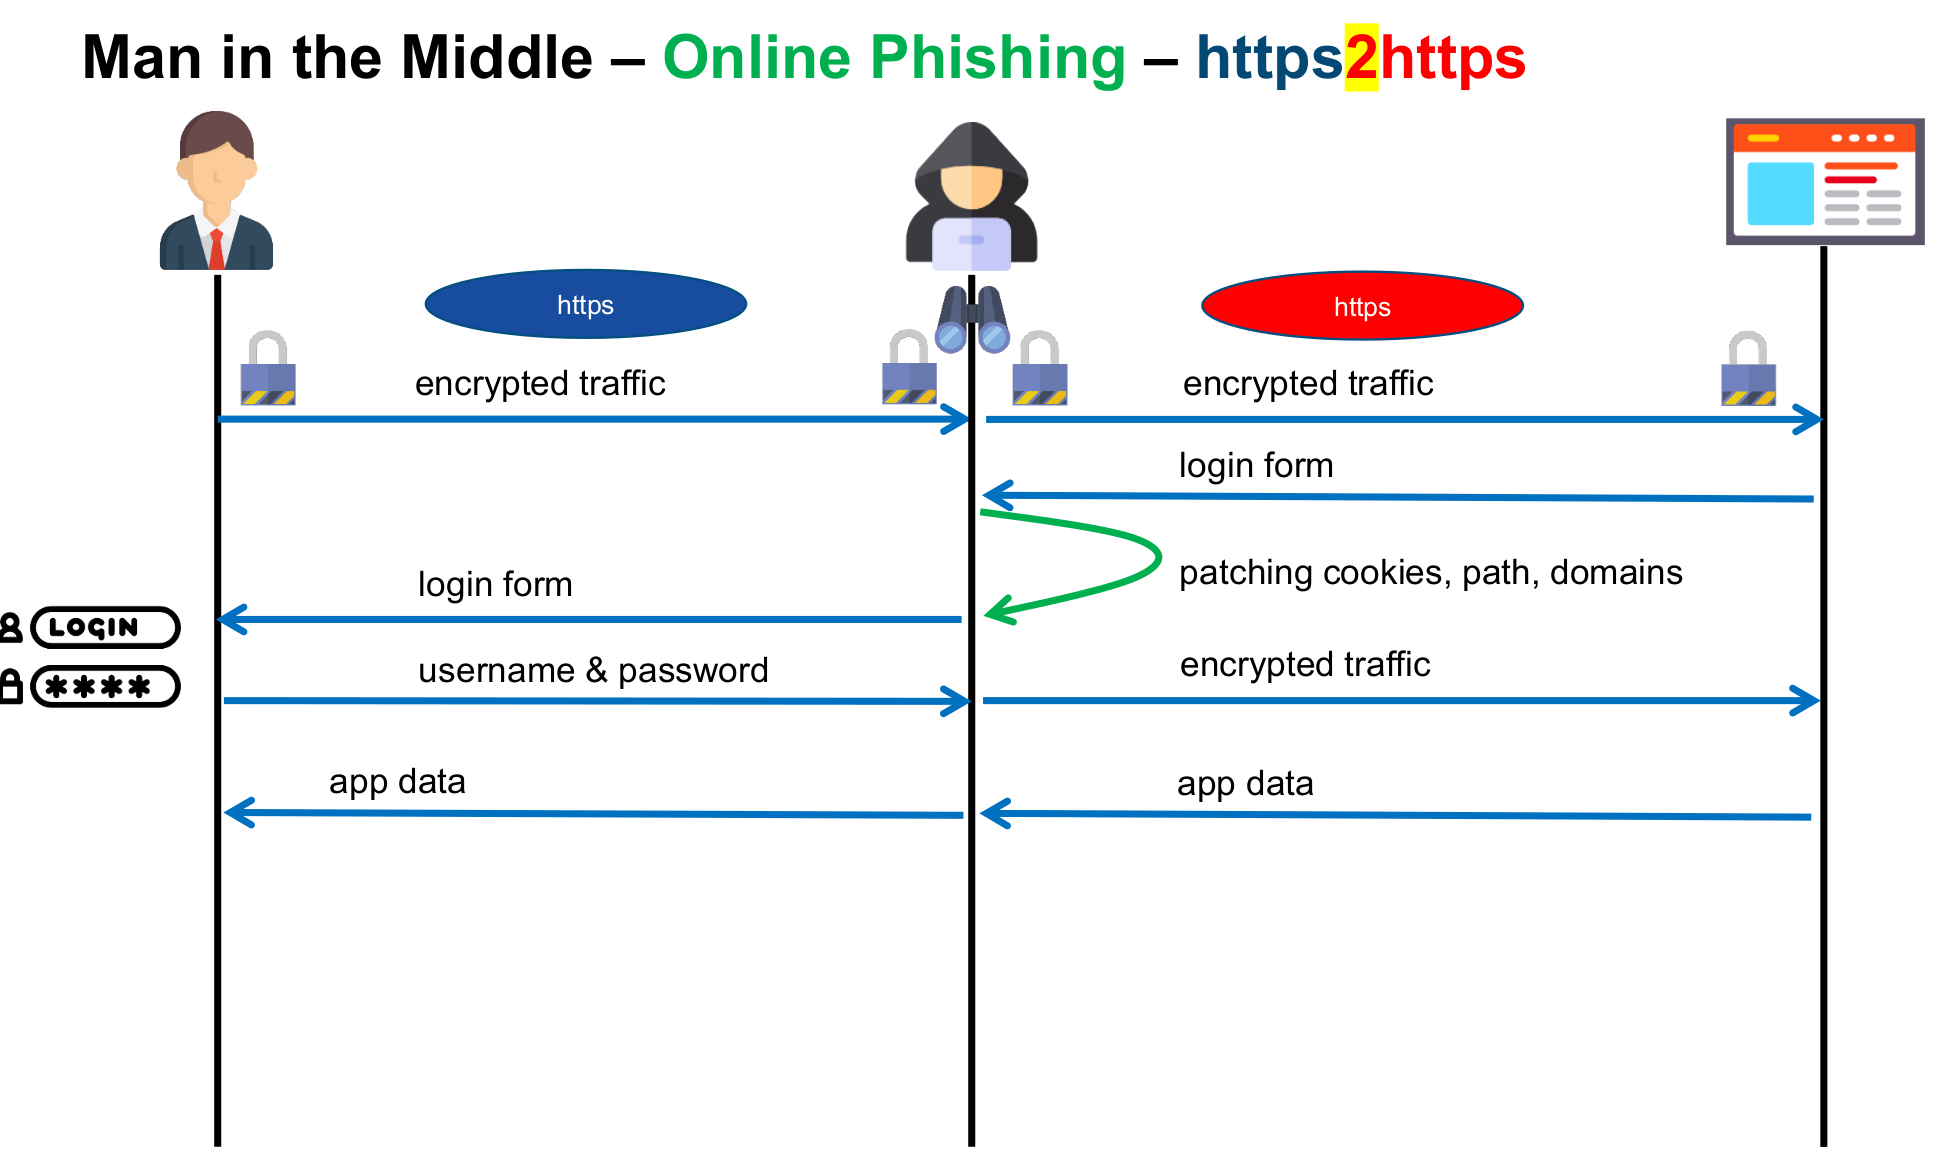
\includegraphics[width=\textwidth]{resources/07-mitm-online-phishing-https2https.png}  
\end{center}
\textbf{https2https}
\textbf{Attack Overview}

This is a sophisticated HTTPS-to-HTTPS MITM phishing attack where the attacker intercepts encrypted traffic between the client and server. The attacker maintains two separate HTTPS connections and acts as a proxy, intercepting login credentials while patching cookies, paths, and domains to maintain the illusion of a legitimate connection. All traffic remains encrypted, but the attacker controls both encryption channels.

\textbf{Protocols Involved}
\begin{itemize}
    \item HTTPS/TLS
    \item TCP/IP
    \item HTTP cookies
    \item Session protocols
    \item Authentication protocols
    \item Domain resolution protocols
\end{itemize}

\textbf{Attack Capabilities}
\begin{itemize}
    \item Credential interception despite encryption
    \item Session token manipulation
    \item Cookie hijacking
    \item Path manipulation
    \item Domain spoofing
    \item Real-time traffic manipulation
    \item Authentication bypass
    \item Session riding
\end{itemize}

\textbf{Mitigation Strategies}
\begin{itemize}
    \item Certificate pinning
    \item HSTS implementation
    \item Multi-factor authentication
    \item Certificate transparency monitoring
    \item Token binding
    \item Secure cookie attributes
    \item Domain verification
    \item Client certificate authentication
    \item Extended validation certificates
    \item Security headers (HSTS, CSP, etc.)
\end{itemize}


\begin{center}
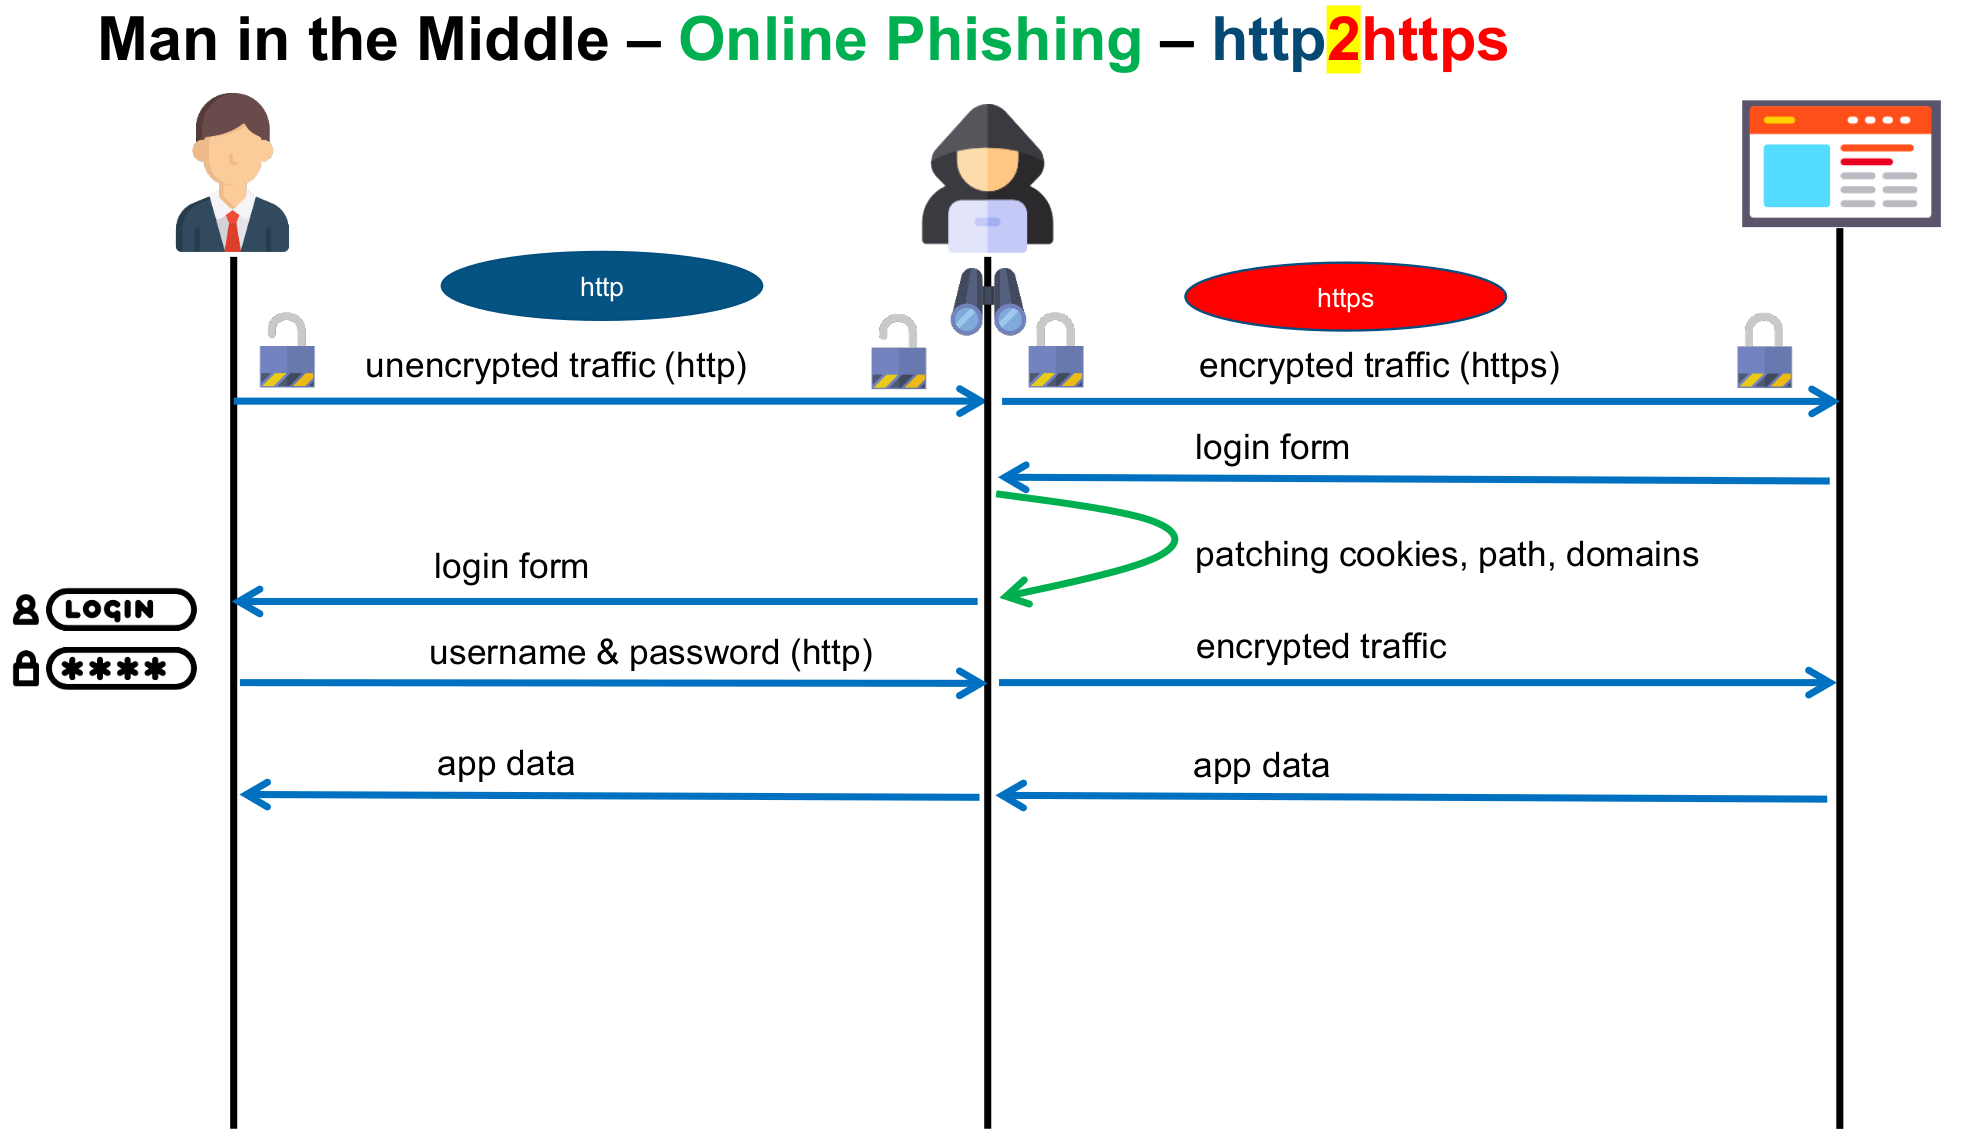
\includegraphics[width=\textwidth]{resources/07-mitm-online-phishing-http2https.png}  
\end{center}
\textbf{Attack Overview}

This attack shows a HTTP-to-HTTPS MITM scenario where the attacker exploits the unencrypted HTTP connection from the client while maintaining an encrypted HTTPS connection to the server. The victim's credentials are transmitted in plaintext on the HTTP side, while the attacker maintains a legitimate HTTPS connection with the target server, effectively bypassing the server's encryption requirements.

\textbf{Protocols Involved}
\begin{itemize}
    \item HTTP (client side)
    \item HTTPS/TLS (server side)
    \item TCP/IP
    \item Cookie handling protocols
    \item Authentication protocols
    \item Domain protocols
\end{itemize}

\textbf{Attack Capabilities}
\begin{itemize}
    \item Plaintext credential interception
    \item Session cookie manipulation
    \item Domain spoofing
    \item SSL stripping
    \item Authentication bypass
    \item Path manipulation
    \item Traffic inspection
    \item Cookie hijacking
\end{itemize}

\textbf{Mitigation Strategies}
\begin{itemize}
    \item HSTS implementation
    \item HSTS preloading
    \item Automatic HTTPS redirection
    \item Secure cookie attributes
    \item TLS everywhere
    \item CSP enforcement
    \item Certificate pinning
    \item Multi-factor authentication
    \item Strict transport security
    \item Force HTTPS for all connections
\end{itemize}

\subsection{HTTPS MitM Mitigation}
\begin{itemize}
  \item Certification Transparency
  \item HSTS
  \item SSL/TLS \& Mutual Authentication \newline
  \begin{center}
    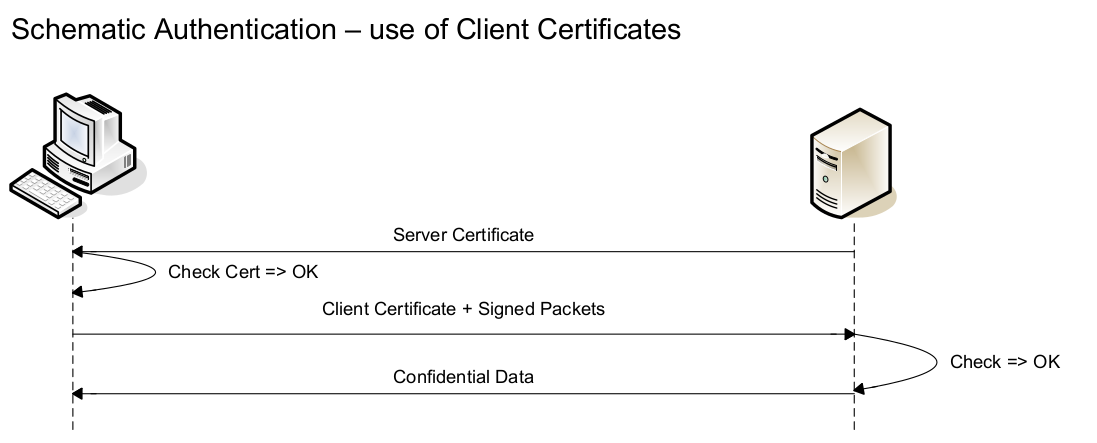
\includegraphics[width=\textwidth]{resources/07-https-mitam-mitigation-ssl.png} 
    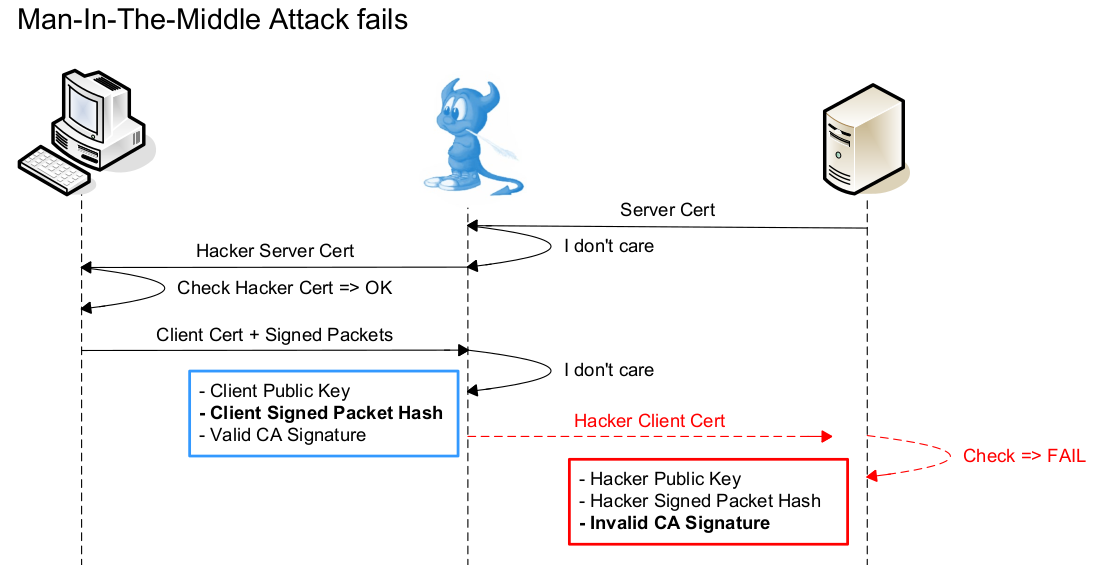
\includegraphics[width=\textwidth]{resources/07-https-mitam-mitigation-ssl-2.png} 
  \end{center}
  \item FIDO Challenge Response Protocol \newline
  \begin{center}
    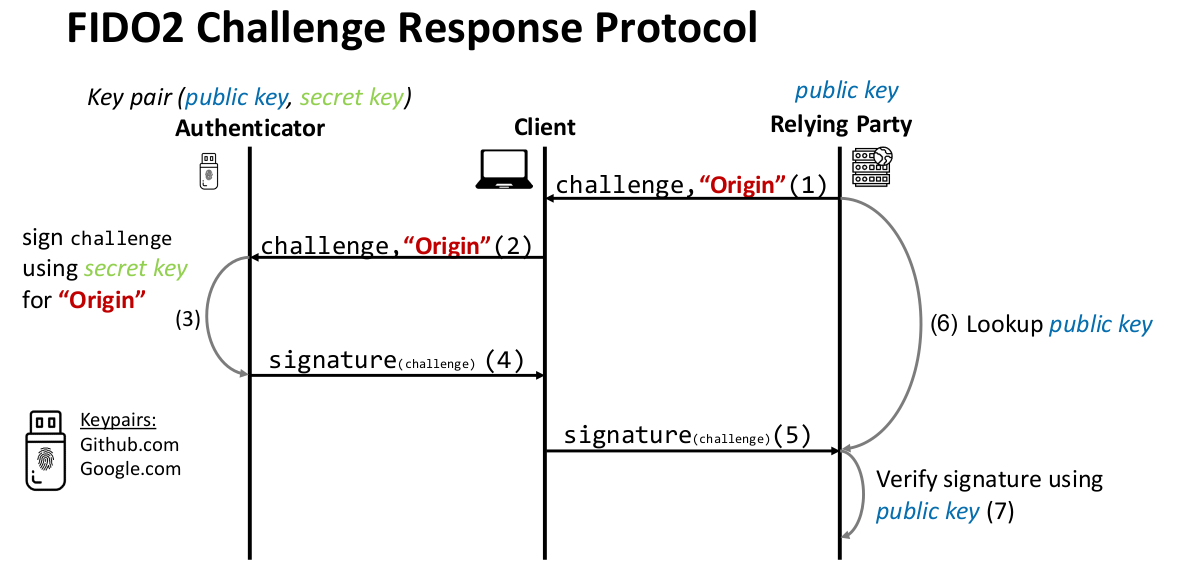
\includegraphics[width=\textwidth]{resources/07-https-mitam-mitigation-fido2.png} 
  \end{center}
  \item User Awareness Training
  \item Monitoring similar domain registrations as the own domain (dnstwists)
  \item Being able to block certain websites or domains in case of emergency
\end{itemize}

\subsection{MITM FIDO2}
\subsubsection*{Traditional 2FA}
\begin{itemize}
  \item To \textbf{KNOW} something: Password, Ping
  \item To \textbf{OWN} something: Smartcard, SecureId, Safeword, etc
  \item To \textbf{BE} something: Fingerprint, Iris, Voice, Face
  \item Multi-Factor: 2 \textbf{DIFFERENT} factors
\end{itemize}
Issue: Most second factor mechanisms do not protect against credential phishing.

Here's an explanation of 2FA phishing scenarios:

\textbf{HOTP/TOTP Based 2FA Phishing}
\begin{itemize}
    \item \textbf{Attack Flow:}
        \begin{itemize}
            \item Attacker creates phishing site mimicking legitimate login
            \item User enters credentials on phishing site
            \item Attacker immediately uses these on real site
            \item Real site requests 2FA code
            \item User enters TOTP code on phishing site
            \item Attacker quickly uses this code before it expires
        \end{itemize}
    \item \textbf{Limitations:}
        \begin{itemize}
            \item Time-sensitive (30-60 seconds for TOTP)
            \item Requires real-time relay
            \item One-time use of codes
        \end{itemize}
\end{itemize}

\textbf{Push Notification 2FA Phishing}
\begin{itemize}
    \item \textbf{Attack Flow:}
        \begin{itemize}
            \item User enters credentials on phishing site
            \item Attacker initiates login on legitimate site
            \item Victim receives legitimate push notification
            \item User approves push notification thinking it's their login attempt
            \item Attacker gains access to account
        \end{itemize}
    \item \textbf{Why It Works:}
        \begin{itemize}
            \item Exploits user trust in push notifications
            \item Uses legitimate authentication channel
            \item No code interception needed
            \item Often more successful than TOTP phishing
        \end{itemize}
\end{itemize}

\textbf{Mitigation Strategies}
\begin{itemize}
    \item Number matching in push notifications
    \item Location information in 2FA prompts
    \item FIDO2/WebAuthn implementation
    \item User education about verification
    \item Phishing-resistant authentication methods
    \item Biometric verification requirements
\end{itemize}

\subsubsection{FIDO2 Building Blocks}
\begin{center}
  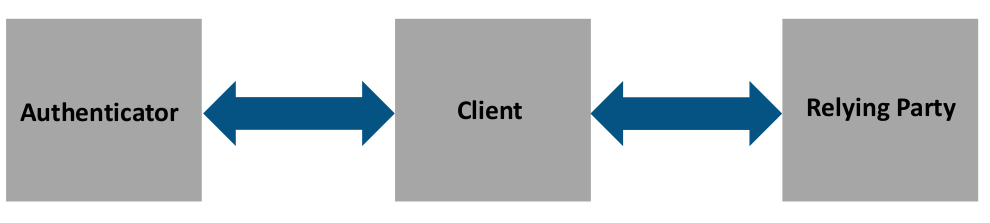
\includegraphics[width=\textwidth]{resources/07-mitm-mitigation-fido2.png}
\end{center}

\textbf{FIDO2 Authenticators}
\textbf{Hardware Authenticators}
\begin{itemize}
    \item YubiKey (various models)
    \item Google Titan Security Keys
    \item Feitian FIDO2 Keys
    \item Thetis FIDO2 Keys
    \item SoloKeys (open source)
    \item NitroKey FIDO2
    \item AuthenTrend Keys
    \item HyperFIDO Keys
\end{itemize}

\textbf{Platform Authenticators}
\begin{itemize}
    \item Windows Hello
    \item Apple Touch ID
    \item Apple Face ID
    \item Android Fingerprint
    \item TPM (Trusted Platform Module)
    \item Intel SGX
\end{itemize}

\textbf{Biometric Authenticators}
\begin{itemize}
    \item Fingerprint sensors
    \item Face recognition systems
    \item Iris scanners
    \item Voice recognition
\end{itemize}

\textbf{By Connection Type}
\begin{itemize}
    \item USB-A
    \item USB-C
    \item NFC
    \item Bluetooth
    \item Lightning (for iOS)
    \item Hybrid (multiple connections)
\end{itemize}

\textbf{Special Purpose Authenticators}
\begin{itemize}
    \item Military-grade authenticators
    \item Enterprise security tokens
    \item Government ID authenticators
    \item Banking-specific tokens
\end{itemize}

\subsection{CTAP Client to Authenticator Protocol}
\textbf{CTAP (Client to Authenticator Protocol)}

CTAP is a core component of FIDO2 that enables communication between authenticators and clients. It consists of two main versions:

\textbf{CTAP1 (formerly U2F)}
\begin{itemize}
    \item Original protocol for FIDO Universal 2nd Factor
    \item Simple challenge-response mechanism
    \item Limited to second-factor authentication
    \item Uses USB HID protocol
    \item Backwards compatible with older security keys
\end{itemize}

\textbf{CTAP2}
\begin{itemize}
    \item Modern protocol with enhanced capabilities
    \item Supports passwordless authentication
    \item PIN/biometric verification
    \item Resident credentials storage
    \item Multiple transport options:
        \begin{itemize}
            \item USB
            \item NFC
            \item Bluetooth Low Energy (BLE)
        \end{itemize}
\end{itemize}

\textbf{Protocol Flow}
\begin{itemize}
    \item Client requests authentication/registration
    \item Platform mediates communication
    \item Authenticator performs cryptographic operations
    \item Response returned via platform to client
\end{itemize}

\textbf{Key Features}
\begin{itemize}
    \item User presence verification
    \item User verification (PIN/biometric)
    \item Credential management
    \item Discovery capabilities
    \item Enterprise attestation
    \item Transaction confirmation
\end{itemize}

\textbf{Security Properties}
\begin{itemize}
    \item Origin binding
    \item Public key cryptography
    \item Protection against phishing
    \item Hardware-backed security
    \item Anti-cloning measures
\end{itemize}

\subsection{WebAuthn}
\textbf{WebAuthn (Web Authentication)}

WebAuthn is a web standard for strong authentication that enables passwordless and second-factor authentication using public-key cryptography.

\textbf{Core Components}
\begin{itemize}
    \item Relying Party (website/application)
    \item Authenticator (FIDO2 device/platform)
    \item Browser/Platform (WebAuthn client)
    \item User Agent (handles interactions)
\end{itemize}

\textbf{Key Operations}
\begin{itemize}
    \item \textbf{Registration (Credential Creation)}
        \begin{itemize}
            \item Website requests credential creation
            \item User consents and authenticates
            \item Authenticator generates key pair
            \item Public key stored on server
            \item Private key securely stored in authenticator
        \end{itemize}
    
    \item \textbf{Authentication (Assertion)}
        \begin{itemize}
            \item Website requests authentication
            \item User proves possession of private key
            \item Challenge-response verification
            \item Server validates response
        \end{itemize}
\end{itemize}

\textbf{Supported Authentication Types}
\begin{itemize}
    \item Platform authenticators (Windows Hello, Touch ID)
    \item Roaming authenticators (Security keys)
    \item Resident credentials (passwordless)
    \item Non-resident credentials (2FA)
    \item User verification (biometric/PIN)
    \item User presence (simple touch)
\end{itemize}

\textbf{Security Features}
\begin{itemize}
    \item Origin binding
    \item Anti-phishing protection
    \item Cryptographic attestation
    \item No shared secrets
    \item No password transmission
    \item Protection against replay attacks
\end{itemize}

\textbf{Implementation Considerations}
\begin{itemize}
    \item Browser compatibility
    \item Authenticator selection
    \item Fallback mechanisms
    \item User experience design
    \item Recovery procedures
    \item Enterprise policies
\end{itemize}

\subsection{Password-Less Authentication}
\textbf{Passwordless Authentication Overview}

This is a modern authentication method that eliminates passwords in favor of stronger, more user-friendly authentication factors.

\textbf{Common Methods}
\begin{itemize}
    \item \textbf{FIDO2/WebAuthn}
        \begin{itemize}
            \item Security keys
            \item Platform authenticators
            \item Biometric verification
        \end{itemize}
    
    \item \textbf{Magic Links}
        \begin{itemize}
            \item Email-based authentication
            \item One-time unique URLs
            \item Time-limited access
        \end{itemize}

    \item \textbf{Biometrics}
        \begin{itemize}
            \item Fingerprint scanning
            \item Facial recognition
            \item Voice authentication
            \item Iris scanning
        \end{itemize}
\end{itemize}

\textbf{Benefits}
\begin{itemize}
    \item Eliminates password-related vulnerabilities
    \item Reduces phishing risks
    \item Better user experience
    \item Lower support costs
    \item Stronger security
    \item Reduced account recovery needs
\end{itemize}

\textbf{Implementation Considerations}
\begin{itemize}
    \item Account recovery procedures
    \item Multiple device support
    \item Backward compatibility
    \item User education
    \item Fallback authentication methods
    \item Cross-platform support
\end{itemize}

\textbf{Security Aspects}
\begin{itemize}
    \item Public key cryptography
    \item Hardware security elements
    \item Biometric data protection
    \item Device attestation
    \item Anti-replay protection
    \item Multiple factor options
\end{itemize}

\subsection{MITM RDP}
Here's a comprehensive breakdown of RDP MITM:

\textbf{RDP Overview}
Remote Desktop Protocol (RDP) is Microsoft's proprietary protocol that provides remote access to Windows systems, allowing users to control a computer over a network connection through a graphical interface.

\textbf{RDP Protocol Components}
\begin{itemize}
    \item TCP port 3389 (default)
    \item X.224 protocol for connection initialization
    \item T.125 MCS protocol for multiplexing
    \item Virtual channels for data transmission
    \item Support for various security layers
\end{itemize}

\textbf{RDP Security Layers}
\begin{itemize}
    \item Standard RDP security (basic)
    \item TLS/SSL encryption
    \item Network Level Authentication (NLA)
    \item CredSSP (Credential Security Support Provider)
    \item Enhanced RDP Security (RDP 10+)
\end{itemize}

\textbf{PyRDP}
\begin{itemize}
    \item Python-based RDP man-in-the-middle tool
    \item Capabilities:
        \begin{itemize}
            \item Session monitoring
            \item Credential capturing
            \item File transfer interception
            \item Recording sessions
            \item Live playback
        \end{itemize}
    \item NLA bypass: Cannot directly bypass NLA, but can exploit misconfigured systems or downgrade attacks
\end{itemize}

\textbf{RDP Protocol Stack}
```
Application Layer
    |
Security Layer (TLS/CredSSP)
    |
MCS Layer (T.125)
    |
X.224 Layer
    |
TCP/IP
```

\textbf{CredSSP Handshake with NTLM}
\begin{itemize}
    \item Initial TLS connection establishment
    \item SPNEGO negotiation
    \item NTLM challenge-response:
        \begin{itemize}
            \item NTLM\_NEGOTIATE
            \item NTLM\_CHALLENGE
            \item NTLM\_AUTHENTICATE
        \end{itemize}
    \item Credential delegation
    \item Session key establishment
\end{itemize}

\textbf{CredSSP with NTLM Authentication Flow}
\begin{itemize}
    \item Client initiates CredSSP
    \item TLS tunnel established
    \item NTLM over TSRequest messages
    \item Server authentication
    \item Credential verification
    \item Public key validation
    \item Session establishment
\end{itemize}

\textbf{MITM Attack Vectors}
\begin{itemize}
    \item SSL/TLS interception
    \item Protocol downgrade attacks
    \item Credential harvesting
    \item Session hijacking
    \item Certificate spoofing
    \item NLA bypass attempts
\end{itemize}

\textbf{Mitigation Strategies}
\begin{itemize}
    \item Enforce NLA
    \item Use strong TLS configurations
    \item Certificate validation
    \item Network segmentation
    \item Access control lists
    \item Regular security updates
    \item Monitoring for suspicious connections
\end{itemize}

\section{exercise}
